\documentclass{article}

\usepackage{ctex}
\usepackage{tikz}
\usetikzlibrary{calc}
\usetikzlibrary{cd}
\usetikzlibrary{decorations.pathreplacing}

\usepackage{amsthm}
\usepackage{amsmath}
\usepackage{amssymb}

\usepackage{hyperref} %url
\hypersetup{
    colorlinks=true,
    linkcolor=blue,
    filecolor=magenta,      
    urlcolor=cyan,
    pdftitle={Overleaf Example},
    pdfpagemode=FullScreen,
    }

\usepackage{enumitem}

\usepackage[textwidth=18cm]{geometry} % 设置页宽=18

\usepackage{blindtext}
\usepackage{bm}
\parindent=0pt
\setlength{\parindent}{2em} 
\usepackage{indentfirst}



\usepackage{xcolor}
\usepackage{titlesec}
\titleformat{\section}[block]{\color{blue}\Large\bfseries\filcenter}{}{1em}{}
\titleformat{\subsection}[hang]{\color{red}\Large\bfseries}{}{0em}{}
%\setcounter{secnumdepth}{1} %section 序号

\newtheorem{theorem}{Theorem}[section]
\newtheorem{lemma}[theorem]{Lemma}
\newtheorem{corollary}[theorem]{Corollary}
\newtheorem{proposition}[theorem]{Proposition}
\newtheorem{example}[theorem]{Example}
\newtheorem{definition}[theorem]{Definition}
\newtheorem{remark}[theorem]{Remark}
\newtheorem{exercise}{Exercise}[section]
\newtheorem{annotation}[theorem]{Annotation}

\newcommand*{\xfunc}[4]{{#2}\colon{#3}{#1}{#4}}
\newcommand*{\func}[3]{\xfunc{\to}{#1}{#2}{#3}}

\newcommand\Set[2]{\{\,#1\mid#2\,\}} %集合
\newcommand\SET[2]{\Set{#1}{\text{#2}}} %

\newcommand{\norm}[1]{\left\lVert#1\right\rVert} % 范数
\newcommand{\vect}[1]{\mathbf{#1}} % vector

\begin{document}
\title{考研高数}
\author{枫聆}
\maketitle
\tableofcontents

\newpage
\section{经典证明}
\begin{theorem}
\rm {\color{red} (Weierstrass第一定理或者连续函数在闭区间上必有界)} 若real-valued函数$f$在闭区间$[a,b]$上连续,那么它在其上有界(上下界).
\end{theorem}

\begin{proof}
{\color{blue} (方法1: 构造$f(x)$非空子区间$[a,x]$,求其上确界)} 假设$B$是使得$f(x)$在形如闭区间$[a,x]$上有界的$x \in [a,b]$集合,显然$a \in B$,所以$B$非空。若$e \in B$且$e > a$,那么$a$和$e$之间的点都是在$B$里面的,所以实际上$B$是一个闭区间. 我们再考虑$B$的上确界,根据$x$的取法,有$x \leq b$,如果我们能证明它的上确界在$b$处取得,那么整个命题就得证. 现在假设$\sup(B) < b$, 由于$B$是一个闭区间,所以$\sup(B) \in B$. 再由于$f$是连续的,那么在充分靠近$\sup(B)$的地方,即$s -\sup(B) < \delta$且$s > \sup(B)$,有$|f(s) - f(\sup(B))| < \varepsilon$,那么$f(x),\;x \in [\sup(B),s]$也是有界,这是和$\sup(B)$是$B$的上确界矛盾的.

{\color{blue} (方法2: 构造一个严格递增的发散数列,其所有子列收敛造矛盾,即Bolzano-Weierstrass定理)}.
\end{proof}

\begin{theorem}
\rm {\color{red} (确界原理)} 任一有上界的非空实数集必有上确界,同理任一有下界的非空实数集必有下确界.
\end{theorem}

\begin{proof}
{\color{blue} (构造一个实数划分,用戴德金分割定理说明界数就是确界)}假设非空实数集$S$有上界$M$,取$S$所有上界为集合$B$. 因为$M \in B$所以$B$非空,取$A = \mathbb{R} \setminus B$,要证明$A$是非空是trivial的,取$x = x_0 - 1,\; x_0 \in S$,那么$x \in A$. 显然地$A$里面所有的元素都小于$B$里面的元素(若是大于$B$里面某个元素,那么它就是$S$的一个上界了,这是矛盾的),这样我们就可以得到一个实数上的划分,根据{\color{red} 戴德金实数分割定理},存在一个$\beta$,它要么是$A$里面最大值或者要么$B$里面的最小值. 假设它是$A$里面的最大值,根据$A$的定义,对于任意$a \in A$都存在一个$x_0 \in S$使得$a < x_0$,将其作用到$\beta$上,我们得到某个$x_0' \in S$使得$\beta < x_0'$. 我们考虑$\frac{x_0'+\beta}{2}$,有
$$
\beta < \frac{x_0' + \beta}{2} < x_0'
$$
所以$\frac{x_0' + \beta}{2} \in A$,这和$\beta$是$A$里面最大值是矛盾的,所以$\beta \in B$,即这个$\beta$就是$S$的上确界.
\end{proof}

\begin{theorem}
\rm {\color{red} (零点定理或者Bolzano-Cauchy第一定理)} 若real-valued函数$f(x)$在闭区间$[a,b]$上定义着并且连续,且$f(a)f(b) < 0$. 则$a$与$b$之间存在一点$c$,使得
$$
f(c) = 0.
$$
\end{theorem}

\begin{proof}
{\color{blue} ($c$是集合的确界) }为方便证明我们假设$f(a) < 0$和$f(b) > 0$,根据$f(x)$在点$a$处连续,根据保号性可知在足够接近$a$的$x$的函数值也都是小于$0$的,我们取集合$S = \Set{x \in [a,b]}{f(x) < 0}$,显然$S$是不为空的,因为$a \in S$,我们考虑$\sup(S)$,记为$c = \sup(S)$. 显然一定也有$c \leq b$. 我们来证明$f(c) = 0$,利用反证法假设$f(c) < 0$,那么由于$f(x)$在$c$点连续,我们在其右边$c+\delta$找到一点$c'$使得$f(c') < 0$,这和$c$的定义是矛盾的,再考虑$f(c) > 0$,同样由于其连续性,同样可以在$c$左边$c-\delta$找到一点$c'$使得$f(c') > 0$,这和$c$的定义还是矛盾的. 所以$f(c) = 0$.

{\color{blue} 另一种证明手法可以使用区间套}.
\end{proof}

\begin{theorem}
\rm {\color{red} (介值定理或者Bolzano-Cauchy第二定理)} 若real-valued函数$f(x)$在区间$\mathcal{X}$上定义着并且连续. 若在$\mathcal{X}$上两点$x=a$和$x=b$处有着不相同的函数值
$$
f(a) = A ~\text{and} ~f(b) = B.
$$
则对于$A$和$B$之间任意的数$C$,均存在一点$c$位于$a$和$b$之间使得
$$
f(c) = C.
$$
用自然语言描述这个性质就是{\color{blue}当连续函数从一个值转变到另一个值时,它必经过每一中间值一次,换句话说就是$x$在$\mathcal{X}$上变动时其对应的函数值将完全充满某一区间$\mathcal{Y}$}.
\end{theorem}

\begin{proof}
为方便证明,我们设$A < C < B$且$a < b$. 在$[a,b]$上考察连续函数$\varphi(x) = f(x) - C$,那么有$\varphi(a) = f(a) - C < 0$和$\varphi(b) = f(b) - C >0$,根据零点定理,我们可以马上得到存在$x=c$使得$\varphi(c) =f(c) - C =0$,即$f(c) = C$.
\end{proof}

\begin{theorem}
\rm {\color{red} (极值定理或者Weierstrass第二定理)} 若real-valued函数$f$在闭区间$[a,b]$连续,那们存在$c,d \in [a,b]$使得
$$
f(c) \leq f(x) \leq f(d),\; x \in [a,b].
$$
\end{theorem}

\begin{proof}
{\color{blue} (构造一个特殊连续函数说明原函数可以取到确界)}$f$在闭区间$[a,b]$上连续({\color{red} 连续闭有界}),那么马上可以得到$f$在$[a,b]$上有界. 取集合$Y = \Set{f(x)}{ x \in [a,b]}$,即$Y$有界,根据{\color{red}确界原理} $Y$有确界,那么我们下面证明思路,就是看$f(x)$是不是能取到这个确界. 取其上确界为$m$,假设不存在$d \in [a,b]$使得$f(d) = m$,那么我们考虑函数$g(x)=\frac{1}{m - f(x)}$,由于$m > f(x),\; x \in [a,b]$,所以$g(x)$在$[a,b]$上是连续的,又因为$f$在$[a,b]$是上有界的,那么$g$在其上也是有界的. 由于$m$是上确界,所以对任意的正实数$\varepsilon$,都有$m - f(x) \leq \varepsilon$,那么$g(x) \geq \frac{1}{\varepsilon}$,这说明$g(x)$是发散的,造成了矛盾. 所以$f$是可以取到上确界的.
\end{proof}

\begin{lemma}
\rm {\color{red} (方便证明费马定理的小引理)} 设real-valued函数$f(x)$在点$x_0$处有有限导数$f'(x_0)$. 若$f'(x_0) > 0\left[ f'(x_0) < 0\right]$,则当$x$取右方充分接近$x_0$的数时就有$f(x) > f(x_0)\left[ f(x) < f(x_0)\right]$,而当$x$取左方充分接近于$x_0$的数值时就有$f(x) < f(x_0)\left[ f(x) > f(x_0)\right]$.
\end{lemma}

\begin{proof}
{\color{blue}这里就需要考虑单侧导数},若$f(x_0) > 0$,依据导数的定义
$$
\frac{f(x) - f(x_0)}{x - x_0},
$$
若$x$从左边接近$x_0$,那么有$x-x_0  < 0$,那么必然有$f(x)-f(x_0) < 0$ ($x$充分接近$x_0$). 同理$x$从右边接近$x_0$,那么$x- x_0 > 0$,必然也有$f(x)-f(x_0) > 0$ ($x$充分接近$x_0$).
\end{proof}

\begin{theorem}
\rm {\color{red} (费马定理)} 设real-valued函数是在某一区间$\mathcal{X}$上定义着,并且在这区间的内点$c$ (存在一个$\mathcal{X}$的子开区间包含$c$) 取得最大(最小值). 若在这点处存在着有限导数$f'(c)$,则必有$f'(c) = 0$.
\end{theorem}

\begin{proof}
方便证明,假设$f(x)$在$c$点取得最大值. 分情况考虑,若$f'(c) > 0$,那么在其$c$左边充分接近$c$的函数值$f(x) > f(c)$,这其最大值的含义矛盾. 同理若$f'(c) < 0$,那么在其$c$的右边充分接近$c$的函数值$f(x) > f(c)$,也是和其最大值矛盾的. 故$f'(c) = 0$.
\end{proof}

\begin{theorem}
\rm {\color{red} (达布定理)} 若real-valued函数$f(x)$在闭区间$[a,b]$内有有限导数,则$f'(x)$必至少有一次取得介于$f'(a)$及$f'(b)$之间的值.
\end{theorem}

\begin{proof}
{\color{blue} 第一想法肯定是特别想用连续函数的介值定理,但是用不了,这里并没有条件说明$f'(x)$是连续的},特别地{\color{red}可导不一定代表其导函数连续},i.e. $x^2 \sin\frac{1}{x}$ . 首先证明若$f'(a)$和$f'(b)$异号时,必有$c \in (a,b)$使得$f'(c)=0$,方便证明不是一般性设$f'(a) < 0$和$f'(b) > 0$,$f(x)$可导即连续,根据{\color{red}极值定理},存在一点$c$使得$f(c)$为最大值,根据前面的{\color{red}费马定理},这个最大值必不可能在$a$或者$b$点取到,因此$c \in (a,b)$且$f'(c)=0$.

再来考虑一般情况,取位于$f'(a)$和$f'(b)$之间任意的$C$,方便证明设$f'(a) < C < f'(b)$. 考虑函数$\varphi(x) = f(x) - Cx$,它的导数为$\varphi'(x) = f'(x) - C$,特别地有$\varphi'(a) < 0$和$\varphi'(b) > 0$,即回到了我们刚开始考虑的情况,所以存在一点$c \in (a,b)$使得$\varphi'(c) = f'(c) - C =0$.
\end{proof}

\begin{theorem}
\rm {\color{red} (罗尔定理)}如果real-valued函数$f$在闭区间$[a,b]$上连续,且在开区间$(a,b)$内可导,若有$f(a) = f(b)$,那么存在至少一个$c \in (a,b)$使得
$$
f'(c) = 0.
$$
\end{theorem}

\begin{proof}
{\color{blue} (确界处导数存在的充分必要条件)} 若函数$f$在$[a,b]$上连续,那么根据{\color{red} 极值定理}其在$[a,b]$是可以取到极值的,分两种情况讨论: (1 如果其最大值和最小值同时在$a,b$取得,那么$f$就是常函数,对任意的$x \in [a,b]$都有$f'(x) = 0$. (2 不失一般性,我们假设$f$在一点$c \in (a,b)$处$f(c)$为最大值(若是最小值,考虑$-f$即可),我们来考虑$c$的一个邻域$(c-\varepsilon, c+\varepsilon)$两边,其中$c-\varepsilon$和$c+\varepsilon$均在$[a,b]$里面. 对任意的$h \in (c-\varepsilon, c)$都有
$$
f'(c^-) = \lim\limits_{h \rightarrow c^-}\frac{f(c)- f(h)}{c-h} \leq 0. 
$$
同理对任意的$t \in (c,c+\varepsilon)$都有
$$
f'(c^+) = \lim\limits_{t \rightarrow c^+}\frac{f(t)-f(c)}{t-c} \geq 0.
$$
由于$f$在$c$点可导,那么$f'(c) = f'(c^-) = f'(c^+) = 0$.
\end{proof}


\begin{theorem}
\rm {\color{red} (拉格朗日中值定理)} 若real-valued函数$f$在闭区间$[a,b]$($a < b$)上连续,且在$(a,b)$上可导,那么存在一个实数$c \in (a,b)$使得
$$
f'(c) = \frac{f(b) - f(a)}{b-a}
$$ 
\end{theorem}

\begin{proof}
{\color{blue} (中值定理是罗尔定理的推广)} 构造函数$g(x) = f(x) - rx$,通过选择合适的$r$,使得$g(a) = g(b)$,即
$$
\begin{array}{ll}
g(a) = g(b) &\Leftrightarrow f(a) - ra = f(b) - rb \\
			&\Leftrightarrow r = \frac{f(b) - f(a)}{b-a}.
\end{array} 
$$
那么根据{\color{red} 罗尔定理},我们知道存在一点$c \in (a,b)$,使得$g'(c) = 0$,
$$
\begin{array}{ll}
g'(x) = f'(x) - r \\
g'(c) = f'(c) - r = 0 \\
f'(c) = r = \frac{f(b) - f(a)}{b-a}.
\end{array}  
$$
证毕.
\end{proof}


\begin{theorem}
\rm {\color{red} (柯西中值定理)} 若两个real-valued函数$f$和$g$都在闭区间$[a,b]$($a < b$)上连续,且都在$(a,b)$上可导. 那么存在一点$c \in (a,b)$,使得
$$
(f(b) - f(a))g'(c) = (g(b) - g(a))f'(c). 
$$
特别地,若$g(b) \neq g(a)$且$g'(c) \neq 0$,等价于
$$
\frac{f'(c)}{g'(c)} = \frac{f(b)-f(a)}{g(b) - g(a)}.
$$
\end{theorem}

\begin{proof}
{\color{blue} (柯西中值定理是中值定理的扩展)} 构造函数$h(x) = f(x) - rg(x)$,选择合适$r$使得$h(a) = h(b)$,若$g(b) \neq g(a)$即$r = \frac{f(b)-f(a)}{g(b) - g(a)}$,那么根据{\color{red}罗尔定理}可以得到$h'(c) = 0$, 即
$$
0 = g'(c) - rf'(c) = f'(c) -  \frac{f(b)-f(a)}{g(b) - g(a)}g'(x).
$$
若$g(a) = g(b)$,同样根据{\color{red}罗尔定理}有$g'(c) = 0$,这个条件显然是使得前面第一个等式成立的.
\end{proof}


\begin{theorem}
\rm {\color{red} (夹逼准则)} 若函数$f,g,h$均在以点$a$为聚点的区间$I$上定义着,且对任意的$x \in I$,其中$x \neq a$都有
$$
g(x) \leq f(x) \leq h(x),
$$
并且同时满足
$$
\lim\limits_{x \rightarrow a}g(x) = \lim\limits_{x \rightarrow a}h(x) = L.
$$
那么$\lim\limits_{x \rightarrow a}f(x) = L$.
\end{theorem}

\begin{proof}
{\color{blue} (经典两边夹)} 取任意的正实数$\varepsilon > 0$,根据极限地定义对$g(x)$和$h(x)$我们可以分别找到$|x| < \delta_1$和$|x| < \delta_2$,使得
$$
L-\varepsilon < g(x) < L + \varepsilon~\text{和}~L-\varepsilon < h(x) < L + \varepsilon
$$
成立,我们取$\delta = \min(\delta_1, \delta_2)$,那么当$|x| < \delta$时有
$$
L-\varepsilon < g(x) \leq f(x) \leq h(x) < L+\varepsilon.
$$
由于$\varepsilon$的任意性,所以有$\lim\limits_{x \rightarrow a} f(x) = L$.
\end{proof}

\newpage
\section{数列极限}

\subsection{数列极限的定义}

\begin{definition}
\rm 若对于每一整数$\varepsilon$,不论它怎样小,恒有序号$N$,使在$n > N$时,一切$x_n$满足不等式\[|x_n-a| < \varepsilon\],则称常数$a$为数列$(x_n)$当$n$趋向于无穷时的{\color{red}极限},记为$\lim\limits_{n \rightarrow \infty}=a$. 也可以说这个序列收敛于$a$.
\end{definition}

\subsection{数列极限的几何意义}

\subsection{数列左右极限}

\subsection{数列极限的基本性质}
%局部性
\begin{proposition}
\rm 若$\lim x_n = a$,又$a > p$,那么存在某个正整数$N$,当$n > N$时,一切$x_n$都满足$x_n > p$.
\end{proposition}

%包号性
\begin{proposition}
\rm 若$\lim x_n = a$,有$a > 0$,那么存在某个正整数$N$,当$n > N$时,一切$x_n$都满足$x_n > 0$.
\end{proposition}

%保值性?
\begin{proposition}
\rm 若$\lim x_n = a$,且$a \neq 0$,则必有充分远的$x_n$值,其绝对值大于某个正数$r$:
$$
|x_n| > r > 0 \; (n > N).
$$
{\color{blue} 性质1的推论}.
\end{proposition}

%有界性
\begin{proposition}
\rm 若$\lim x_n = a$,则$(x_n)$必有界.
\end{proposition}

\begin{proof}
我们知道任意给定一个$\varepsilon > 0$,可以找到正整数$N$,使得当$n > N$时的一切$x_n$都满足$ a-\varepsilon < x_n < a + \varepsilon$,因此当$n > N$是存在一个界数使得$|x_n| < M$. 接着再考虑$n \leq N$时,注意这时候只有有限个$x_n$,我们把$M$和它们放在一起,取它们里面绝对值最大的数$M'$,即有$|x_n| \leq M'$.
\end{proof} 

%极限唯一
\begin{proposition}
\rm 若同时有$\lim x_n = a,\; \lim x_n = b$,则$a = b$.  
\end{proposition}

\subsection{数列无穷小和无穷大}

\subsection{数列极限运算}

\begin{proposition}
\rm 若$x_n = y_n$,则$\lim x_n = \lim y_n$.
\end{proposition}

\begin{proposition}
\rm 若恒有$x_n \leq y_n$,且各自趋于有限极限,则$\lim x_n \leq \lim y_n$.
\end{proposition}

\begin{proposition}
\rm {\color{red} 夹闭准则} {\color{blue} 见经典证明}.
\end{proposition}

\begin{proposition}
\rm 任意有限个无穷小的和亦是无穷小.
\end{proposition}

\begin{proposition}
\rm 有界数列$(x_n)$与无穷小${\alpha_n}$的乘积仍是无穷小.
\end{proposition}

\begin{proposition}
\rm 若$\lim x_n = a,\; \lim y_n =b$,则$\lim(x_n\pm y_n) = a \pm b$. 考虑两个极限的尾巴
$$
\lim (x_n \pm y_n) = a+b+ \alpha + \beta.
$$
\end{proposition}

\begin{proposition}
\rm 若$\lim x_n = a,\; \lim y_n =b$,则$\lim(x_ny_n) = ab$. 考虑两个极限的尾巴
$$
\lim x_ny_n = ab + a\beta + b\alpha + \alpha\beta.
$$
\end{proposition}


\begin{proposition}
\rm 若$\lim x_n = a,\; \lim y_n =b$,且$b\neq 0$,则$\lim \frac{x_n}{y_n} = \frac{a}{b}$. 考虑两个极限的尾巴
$$
\lim \frac{x_n}{y_n} = \frac{a+\alpha}{b+\beta}.
$$
\end{proposition}

\subsection{不定式}

\begin{annotation}
$$
\frac{x_n}{y_n} \sim \frac{0}{0}
$$
\end{annotation}

\begin{annotation}
$$
\frac{x_n}{y_n} \sim \frac{\infty}{\infty}
$$
\end{annotation}

\begin{annotation}
$$
x_n y_n \sim  0 \cdot \infty
$$
\end{annotation}

\begin{annotation}
$$
x_n - y_n \sim \infty - \infty
$$
\end{annotation}

\subsection{单调数列的极限}

\begin{theorem}
\rm 给定单调增加的数列$(x_n)$,若它有上界
$$
x_n \leq M,\; n = 1,2,\cdots
$$
则它必有一有限极限,此极限为上确界. 同理单调减少的数理$(x_n)$,若它有下界
$$
x_n \geq M, \; n = 1,2,\cdots
$$
则它必有一有限极限,此极限为下确界.
\end{theorem}

\subsection{收敛原理}

\begin{theorem}
\rm {\color{red} (柯西收敛原理)}数列$(x_n)$有有限极限的必要且充分条件是: 对于任意的数$\varepsilon > 0$,总存在着整数$N$,使得当$n > N$和$n' > N$时有下面不等式成立
$$
|x_n - x_{n'}| < \varepsilon.
$$
\end{theorem}

\begin{proof}
{\color{red} (必要性)} 若$\lim x_n = a$,即对任意的$\frac{\varepsilon}{2}$,能找到一个整数$N$,使得$n, n' > N$时有
$$
|x_n - a| < \frac{\varepsilon}{2},\; |x_{n'} - a| < \frac{\varepsilon}{2}
$$
成立. 那么
$$
|x_n - x_{n'}| = |(x_n -a ) + (a - x_{n'})| \leq |x_n-a| + |x_{n'}-a| < \varepsilon
$$

{\color{red} (充分性)} 若满足上述定理中的条件,{\color{blue}我们要证明$\lim x_n = a$,我们得想办法把这个$a$表示出来,这里手法将会用戴德金实数划分的结论来把这个$a$弄出来}.

在全体实数域下构造一个划分. 对于任何实数$\alpha$,若$x_n$从某项其满足不等式\[x_n > \alpha,\]则取这种实数$\alpha$归入下组$A$,其余的(即不落在$A$里面的)一起实数归入上组$A'$.

首先我们来说明这样确实产生了一个实数上的划分. 由前提条件,对于任意数$\varepsilon>0$及其对应的$N$. 若$n > N$及$n' > N$,则下面不等式成立\[x_{n'} - \varepsilon < x_n < x_{n'}+\varepsilon.\]现在我们可以看到每一个数$x_{n'} - \varepsilon$都是小于$x_n$的,所以它归入下组$A$. 另一方面$x_{n'}+\varepsilon$都大于$x_n$,所以$x_{n'}+\varepsilon$放不进去$A$,那它只能归入$A'$了,所以$A$和$A'$都是非空的. 我们的划分方式对于每一个数$\alpha$和确定序列$x_n$,要么它属于$A$或者属于$A'$. 同时$A$中实数都小于$A'$的实数. 如果$\alpha > \alpha', \alpha \in A , \alpha' \in A'$,则$x_n$从某一项其也都大于$a'$,这样就产生矛盾了. 因此的确产生了一个实数上的划分.

根据戴德金基本定理,有实数$a$存在它是$A$和$A'$的界数,即\[\alpha \leq a \leq \alpha', \; \alpha \in A,\alpha' \in A'.\]我们注意到当$n > N$时,$x_{n'} - \varepsilon$是一个$\alpha$,而$x_{n'} +\varepsilon$是一个$\alpha'$. 所以我们有\[x_{n'} - \varepsilon \leq a \leq x_{n'} + \varepsilon.\]即$|x_{n'}-a| \leq \varepsilon$,所以$\lim x_n = a$.

{\color{blue} 若是不用实数划分的手法,也可以构造$a_n = \inf\limits_{k \geq n} x_k$和$b_n=\sup\limits_{k \geq n}$,证明$\lim a_n = \lim b_n = c$,再用一下夹逼准则$a_n \leq x_n \leq b_n$.}
\end{proof}

\subsection{上下极限}
%https://en.wikipedia.org/wiki/Limit_inferior_and_limit_superior
\begin{definition}
\rm 序列$(x_n)$的部分极限的最大值和最小值,称为$x_n$的上极限和下极限,各记为
$$
\overline{\lim} x_n~\text{及}~\underline{\lim} x_n.
$$
\end{definition}

\newpage
\section{函数极限}

\subsection{函数极限的定义}

\subsection{函数左右极限}

\subsection{用数列的语言来描述函数极限}

\subsection{两个重要极限}

\begin{proposition}
$$
\lim\limits_{x \rightarrow 0} \frac{\sin x}{x}.
$$
\end{proposition}

\begin{proof}
几何证明的手法,或者直接上洛必达.
\end{proof}

\begin{proposition}
$$
\lim\limits_{x \rightarrow +\infty} (1+\frac{1}{x})^x.
$$
\end{proposition}


\begin{proof}
单调有界.
\end{proof}

\subsection{函数极限的基本性质}

%局部性
%保号性
%有界性
\begin{proposition}
\rm 若$\lim\limits_{x \rightarrow a} = A$,则对于充分接近$a$的$x$的函数值是有界的
$$
|f(x)| \leq M ,\; |x-a| < \delta.
$$
{\color{blue} 注意这里和$\lim x_n = b$,而导致整个$(x_n)$有界是区别的,因为这里当$x-a < -\delta$或者$x-a > \delta$可能有无限多个函数值的,它们是否有界是无法确定的}.
\end{proposition}

\subsection{函数极限运算}

\begin{proposition}
\rm 若$\lim\limits_{x \rightarrow a} f(x) = A$和$\lim\limits_{x \rightarrow a} g(x) = B$,则函数
$$
\begin{array}{ll}
\lim\limits_{x \rightarrow a} (f(x) \pm  g(x)) &= A \pm B,\\
\lim\limits_{x \rightarrow a} f(x) \cdot g(x) & = A\cdot B, \\
\lim\limits_{x \rightarrow a} \frac{f(x)}{g(x)} &= \frac{A}{B}.
\end{array}
$$
\end{proposition}

\subsection{不定式}

\begin{annotation}
$$
\frac{0}{0},\; \frac{\infty}{\infty},\; 0\cdot \infty,\; \infty-\infty.
$$
\end{annotation}

\subsection{单调函数的极限}

\begin{theorem}
\rm 若单调增大函数$f(x)$在区域$\mathcal{X}$内变动着. 区域$\mathcal{X}$以大于一切$x$值的数$a$(它可以是有限的数,或者等于$+\infty$)作为聚点,若在这时函数$f(x)$在$\mathcal{X}$上有上界
$$
\forall x \in \mathcal{X},\;f(x) \leq M.
$$
则当$x \rightarrow a$时$f(x)$有一有限极限. 
\end{theorem}

\begin{proof}
若$f(x)$上有界,考虑$f$在$\mathcal{X}$上变动构成的集合$\{f(x)\}$,即$\{f(x)\}$是有上界的,那么根据确界原理,$\{f(x)\}$有上确界,设其为$A$,接下来我们证明$A$就是$f(x)$趋向于$a$的极限.

给定任意$\varepsilon > 0$,根据上确界的性质,可以找到一个$x' < a$,使得$f(x') > A-\varepsilon$. 再由于$f(x)$是单调增的,所以当$x > x'$时,都有$f(x) > A -\varepsilon$,其上界也很容易得到$f(x) \leq A < A+\varepsilon$,所以综上当$x > x'$有
$$
A-\varepsilon < f(x) < A+\varepsilon.
$$
这里$\delta$的取值取决于$a$的取值,若$a$是一个有限的数,那么$\delta = a-x'$即可,若$a = +\infty$,则取$\Delta = x'$. 
\end{proof}

\subsection{函数收敛的判定方法}

\begin{theorem}
\rm 函数$f(x)$当$x$趋于$a$时有一有限极限的充分必要条件为,对于任意$\varepsilon > 0$必存在着$\delta > 0$,只需要满足
$$
|x-a| < \delta,\; |x'-a| < \delta.
$$
就能使得下面不等式成立
$$
|f(x)-f(x')| < \varepsilon.
$$
\end{theorem}

\begin{proof}
{\color{blue}充分性显然,必要性可以通过用数列描述函数极限的方法,配合数列中有限极限存在的充要来条件来进行证明}.
\end{proof}

\subsection{无穷小及无穷大的分阶}


\begin{definition}
\rm 给定两个无穷小$\alpha$和$\beta$
\begin{enumerate}
	\item 若$\frac{\beta}{\alpha}$有一异于零的有限极限,则称$\alpha$和$\beta$是{\color{red}同阶无穷小};
	\item 若$\frac{\beta}{\alpha}$趋于无穷小,则称$\beta$是$\alpha$的{\color{red} 高阶无穷小},记做$\beta = o(\alpha)$.
	同时$\alpha$是$\beta$的低阶无穷小;
\end{enumerate}
\end{definition}

\begin{definition}
\rm 为了更精确地比较无穷小的性态,需要用数字来表示它们的阶,在这种情形下,我们首先在所研究的无穷小内选出一个作为一种"标准",把它称为{\color{red}基本无穷小}.
\end{definition}

\begin{definition}
\rm 若$\beta$与$\alpha^k$是同阶的无穷小量,则称$\beta$是基本无穷小$\alpha$的$k$阶无穷小.
\end{definition}

\begin{definition}
\rm 给定两个无穷小$\alpha$和$\beta$,若它们的差$\gamma = \beta - \alpha$是比$\alpha$和$\beta$中任何一个更高阶的无穷小,则称$\alpha$和$\beta$为{\color{red}等价无穷小},记做$\alpha \sim \beta$.
\end{definition}

\begin{proposition}
\rm 给定两个无穷小$\alpha$和$\beta$,若它们是等价无穷小当且仅当$\lim \frac{\beta}{\alpha} = 1$.
\end{proposition}

\begin{proof}
经常看见的定义实际是一个充要条件,首先证明充分性,设$\delta = \frac{\beta}{\alpha} - 1$,所以有$\lim \delta = 0$. 那么
$$
\gamma = \delta \alpha,
$$
很容易得到$\lim \frac{\gamma}{\alpha} =\lim \delta = 0$和$\lim \frac{\gamma}{\beta} = \lim \delta = 0$.

若$\alpha$和$\beta$是等价无穷小,那么
$$
\lim \frac{\beta-\alpha}{\alpha} = \lim (\frac{\beta}{\alpha} - 1) = 0,
$$
所以$\lim \frac{\beta}{\alpha} = 1$.
\end{proof}


\begin{definition}
\rm 若选定$\alpha$为基本无穷小,则形如$c\cdot \alpha^k$就被称为{\color{red}最简单的无穷小},其中$c$是一个常数,而$k > 0$. 设$\beta$关于$\alpha$的$k$阶无穷小,即
$$
\lim \frac{\beta}{\alpha^k} = c,
$$
其中$c$是异于零的有限数,则
$$
\lim \frac{\beta}{\alpha^k} = 1,
$$
因此$\beta$和$c\alpha^k$为等价无穷小. 与给定无穷小$\beta$等价的最简单的无穷小$c\alpha^k$被称为$\beta$的{\color{red}主部}.
\end{definition}

\begin{annotation}
\rm 设$\beta \sim c\alpha^k$,即$\beta = c\alpha^k + \gamma$,其中$\gamma = o(c\alpha^k)$. 可以想象,再从$\gamma$也可以分出主部$\gamma = c'\alpha^{k'} + \delta$,其中$k' > k$,而$\delta = o(c'\alpha^{k'})$,余类推. {\color{blue}是不是感觉你可以把泰勒展开式由此推出来? 但是这种方法太低效了,但是它却能帮你更好的理解无穷小的概念}.
\end{annotation}


\subsection{洛必达法则}

\begin{definition}
\rm 若real-value函数$f$和$g$都在去心邻域$\tilde{U}(c,\delta)$可导,有
$$
\lim\limits_{x \rightarrow c} f(x) = \lim\limits_{x \rightarrow c} g(x) = 0 ~\text{或者}~ \lim\limits_{x \rightarrow c} g(x) = \infty,
$$
且对任意$x \in \tilde{U}$都有$g'(x) \neq 0$,同时有$\lim\limits_{x \rightarrow c}\frac{f'(x)}{g'(x)}$存在,那么
$$
\lim\limits_{x \rightarrow c} \frac{f(x)}{g(x)} = \lim\limits_{x \rightarrow c} \frac{f'(x)}{g'(x)}.
$$
\end{definition}

\begin{proof}
首先来看一个比较特殊的情况,除满足上述条件之外,若还满足$f(c) = g(c) = 0$,并且$g'(c) \neq 0$,那么
$$
\lim\limits_{x \rightarrow c}  \frac{f(x)}{g(x)} = \lim\limits_{x \rightarrow c} \frac{f(x) - f(c)}{g(x) - g(c)} = \lim\limits_{x \rightarrow c} \frac{ \frac{f(x) - f(c)}{x-c}}{\frac{g(x) - g(c)}{x-c}} = \frac{f'(c)}{g'(c)} = \lim\limits_{x \rightarrow c} \frac{f'(x)}{g'(x)}.
$$
下面来严格证明分两种情况来证明,由于$\tilde{U}$在$c$这里间断,后面需要频繁使用到柯西中值定理,所以自然地在$\title{U}$的两端来分析,取开区间$\mathcal{I}$以$c$点为端点,且$\mathcal{I} \subset \tilde{U}$. {\color{blue}注意到条件满足对任意的$x \in \mathcal{I}$有$g'(x) \neq 0$,并且$g$在$\mathcal{I}$上是连续的,那么是可以在$\mathcal{I}$里面找到一个足够小的区间使得$g(x)\neq 0$,那这个小区间代替$\mathcal{I}$}. 

我们定义$m(x) = \inf\frac{f'(\alpha)}{g'(\alpha)}$和$M(x) = \sup\frac{f'(\alpha)}{g'(\alpha)}$其中$x \in \mathcal{I}$,$\alpha$取遍$x$和$c$之间的数({\color{blue} 为什么确保可以取到确界? 任意$\alpha$处$f$和$g$导数均有意义}). 在确定$x$之后,我们再取定$x$和$c$之间一点$y$,结合柯西中值定理可以保证在它们之间找到一个$c$使得
$$
 m(x) \leq \frac{f(x) - f(y)}{g(x) - g(y)} = \frac{f'(\alpha)}{g'(\alpha)} \leq M(x).
$$
注意为什么这里可以保证$g(x) - g(y) \neq 0$? 假设存在$g(x) = g(y)$, 那么根据罗尔定理,就存在一点$p$使得$g'(p) = 0$,这是和前提条件$\forall x \in \bar{U},\;g'(x) \neq 0$矛盾的.

{\color{blue}情况一}:$\lim\limits_{x \rightarrow c} f(x) = \lim\limits_{x \rightarrow c} g(x) = 0.$

对任意的$x \in \mathcal{I}$, 取$y$位于$x$和$c$之间,为了得到$\frac{f(x)}{g(x)}$,我们让
$$
m(x) \leq \frac{f(x) - f(y)}{g(x) - g(y)} = \frac{\frac{f(x)}{g(x)} - \frac{f(y)}{g(x)}}{1 - \frac{g(y)}{g(x)}} \leq M(x).
$$
当$y \rightarrow c$时,$\frac{f(y)}{g(x)}$和$\frac{g(y)}{g(x)}$都趋向于$0$,所以
$$
m(x) \leq \frac{f(x)}{g(x)} \leq M(x).
$$

{\color{blue}情况二}:$\lim\limits_{x \rightarrow c} g(x) = \infty.$

对任意的$x \in \mathcal{I}$, 取$y$位于$x$和$c$之间. 如果我们还是用上面的分式,直接尝试把$\frac{f(x)}{g(x)}$构造出来,尝试分式对$y \rightarrow c$取极限的时候,显然是无法处理的. {\color{blue}同时你注意到在当前条件下是对$\lim\limits_{x \rightarrow c} f(x)$是没有特别说明的,言下之意它不会对我们的证明产生影响}. 现在我们考虑把前面分式上下都除以$g(y)$,同时上下取负,即
$$
m(x) \leq \frac{f(y) - f(x)}{g(y) - g(x)} = \frac{\frac{f(y)}{g(y)} - \frac{f(x)}{g(y)}}{1 - \frac{g(x)}{g(y)}} \leq M(x).
$$
那么当$y \rightarrow c$时,$\frac{f(x)}{g(y)}$和$\frac{g(x)}{g(y)}$都是趋于$0$,那么此刻关键是我们如何需要考虑$\lim\limits_{y \rightarrow c}\frac{f(y)}{g(y)}$? 让$S_x = \SET{y}{y~\text{位于}~x~\text{和}~c~\text{之间}}$, 我们取遍$y \in S_x$, 我们可以得到得到一个有界数列$\{\frac{f(y)}{g(y)}\}$({\color{red} 为什么有界? $f$和$g$在$[x,c]$上连续}),我们考虑其上下极限
$$
m(x) \leq \lim\limits_{y \rightarrow c }\inf\frac{f(y)}{g(y)} \leq \lim\limits_{y \rightarrow c }\sup\frac{f(y)}{g(y)} \leq M(x).
$$

当对$m(x)$和$M(x)$也取极限$x \rightarrow c$时,有
$$
\lim\limits_{x \rightarrow c} m(x) = \lim\limits_{x \rightarrow c} M(x) = \lim\limits_{x \rightarrow c} \frac{f'(x)}{g'(x)}.
$$
对{\color{blue}情况一}使用{\color{red} 夹逼准则},可以很快得到$\lim\limits_{x \rightarrow c} \frac{f(x)}{g(x)} = \lim\limits_{x \rightarrow c} \frac{f'(x)}{g'(x)}$. 对{\color{blue} 情况二 }也同样使用{\color{red} 夹逼准则},可以得到
$$
\lim\limits_{y \rightarrow c }\inf\frac{f(y)}{g(y)} = \lim\limits_{y \rightarrow c }\sup\frac{f(y)}{g(y)} = \lim\limits_{x \rightarrow c} \frac{f'(x)}{g'(x)},
$$
上下极限相等可以马上得到$\lim\limits_{x \rightarrow c} \frac{f(x)}{g(x)} = \lim\limits_{x \rightarrow c} \frac{f'(x)}{g'(x)}$. 最终证毕.
\end{proof}

\newpage
\section{函数连续及其间断}

\subsection{函数连续的定义}

\begin{annotation}
\rm {\color{red} (motivation)} 在研究$x$趋向于$x_0$的极限时候,即$\lim\limits_{x \rightarrow x_0} f(x)$,并不要求$x$可以取到$x_0$,即使$f(x_0)$有定义,极限也不依赖它. 自然地,现在我们特别地考虑若$f(x_0)$有定义,且$\lim\limits_{x \rightarrow x_0}f(x) = f(x_0)$,这种情形下我们就说$f$在$x_0$处{\color{red}连续},其他情况下则说$f$在$x_0$这里有{\color{red}间断}. {\color{blue} 函数连续是一个局部的性质}.
\end{annotation}

%严格定义

\subsection{连续函数的算术运算}

\begin{theorem}
\rm 若函数$f(x)$和$g(x)$都在区间$\mathcal{X}$上变动着,且都在点$x_0$处连续,则函数
$$
f(x) \pm g(x),\; f(x)\cdots g(x), \; \frac{f(x)}{g(x)}~(g(x_0) \neq 0)
$$
也在都$x_0$处连续.
\end{theorem}

\begin{proof}
{\color{blue}与相关函数的极限联系起来即可}.
\end{proof}

\subsection{单侧连续和间断分类}

\begin{definition}
\rm {\color{red} (单侧极限) }若$f(x)$在$x_0$处是左(右)连续,只需要满足下面关系式
$$
\begin{array}{ll}
f(x_0^-) = \lim\limits_{x \rightarrow x_0^-} = f(x_0). \\
\left[ f(x_0^+) = \lim\limits_{x \rightarrow x_0^+} = f(x_0) \right]
\end{array}
$$
{\color{blue}用自然语言说就是求极限过程中,我们既可以从左边接近$x_0$,也可以从右边接近$x_0$,于是就有了单侧极限的概念}.
\end{definition}

\begin{theorem}
\rm {\color{red} (连续的充要条件)} 函数$f(x_0)$在点$x_0$处连续当且仅当其左极限和右极限都存在且相等.
\end{theorem}

\begin{definition}
\rm 函数$f(x)$可能在$x_0$处存在两类间断点
\begin{enumerate}
	\item $x_0$处单侧极限存在但是不等于$f(x_0)$,则$f(x)$在$x_0$处有间断点,称其为{\color{red}普通间断点}或者{\color{red}第一类间断点},通常说在$f(x)$在$x_0$处有{\color{red}跃度}.
	\item $x_0$处单侧极限是无穷或者根本不存在,则$f(x)$在$x_0$处有间断点,称其为{\color{red} 第二类间断点}.
\end{enumerate}
\end{definition}

\subsection{单调函数的连续性和间断}

\begin{theorem}
\rm {\color{red} (单调函数上的间断点)} 若单调函数$f(x)$在区间$\mathcal{X}$内有间断点,那么只能是第一类间断点.
\end{theorem}

\begin{proof}
若$f(x)$是单调增的,且在$x_0$处有间断点,那么考虑其左极限,当$x < x_0$时,都有$f(x) < f(x_0)$,即$f(x)$在趋近于$x_0$过程中是有界,那么根据单调函数有界则必有有限极限的定理,则有
$$
\lim\limits_{x \rightarrow x^-} f(x) \leq f(x_0).
$$
若可以取到等号,则$f(x)$在$x_0$处左连续,反之$f(x)$在$x_0$处有跃度,所以是第一类间断点. 同理也可以考虑右极限.
\end{proof}

\begin{theorem}
\rm {\color{red} (单调函数连续性判别)} 若在区间$\mathcal{X}$上的单调函数$f(x)$的函数值都含于区间$\mathcal{Y}$,且把整个$\mathcal{Y}$都填满了,即$\forall y \in \mathcal{Y}$,都存在一个$x \in \mathcal{X}$使得$f(x) = y$,则$f(x)$在$\mathcal{X}$上连续.
\end{theorem}

\begin{proof}
若$f(x)$为单调增的,假设$f(x)$在$\mathcal{X}$在$x_0$处有间断点,即$\lim\limits_{x \rightarrow x_0 ^-} f(x) < f(x_0)$,那么$f(x_0^-)$和$f(x_0)$之间的值,$f(x)$是无法取到的,这和命题是矛盾的,所以$f(x)$在$\mathcal{X}$上连续.
\end{proof}

\subsection{初等函数的连续性}

\subsection{连续函数的复合}

\begin{theorem}
若函数$\varphi(y)$定义在区间$\mathcal{Y}$上,而函数$f(x)$定义于区间$\mathcal{X}$上,且其对应的函数值含于$\mathcal{Y}$. 若$f(x)$在$\mathcal{X}$中的一点$x_0$连续,又$\varphi(y)$在$y_0 = f(x_0)$这一点也是连续的,则复合函数$\varphi(f(x))$在点$x_0$处亦是连续的.
\end{theorem}

\subsection{一致性连续}

\begin{annotation}
\rm 在函数连续的定义中,$\delta$的选择可能不仅仅依赖$\varepsilon$,可能同样依赖于$x_0$的选择,因为函数在每个某个点上变动情况可能不一样,变动的越剧烈,$\delta$的选择可能更小,那么是否存在一种连续性$\delta$的选择只依赖$\varepsilon$呢?一致连续就运营而生了.
\end{annotation}

\begin{definition}
\rm 若对于任一数$\varepsilon > 0$,都能求出$\delta > 0$使得当满足
$$
|x-x_0| < \delta
$$
时,都有$|f(x)-f(x_0)| < \varepsilon$,不论$x_0$及$x$在定义域区间$\mathcal{X}$怎样选择,我们就称$f(x)$在$\mathcal{X}$上{\color{red}一致连续},即$\delta$是适用于一切的$x_0$.
\end{definition}

\begin{annotation}
\rm 一致性也可以表示为在$\mathcal{X}$上任意两个$x$取值,只要它们足够的近,它们对应的函数值也是相对来说足够的近. 
\end{annotation}

\begin{theorem}
\rm {\color{red} (康托定理) }若函数$f(x)$是在闭区间$[a,b]$内定义着而且连续,则它在这区间上也是一致连续的.
\end{theorem}

\begin{corollary}
\rm 若函数$f(x)$在闭区间$[a,b]$上定义着且连续. 则对任意的$\varepsilon > 0$,能求出$\delta > 0$,使得把$[a,b]$分成若干个长度小于$\delta$小区间,那么在每个小区间上$f(x)$的振幅(最大值和最小值的差)将小于$\varepsilon$.
\end{corollary}

\newpage
\section{函数导数}

\subsection{导数定义}

\begin{definition}
\rm 设函数$y=f(x)$在点$x_0$的某个邻域内有定义,当自变量$x$在$x_0$处取得增量$\Delta x$时,相应地,因变量取得增量$\Delta y = f(x_0 + \Delta x) - f(x_0)$. 如果$\frac{\Delta y}{\Delta x}$当$\Delta x$趋近于$0$时极限存在,那么称函数$y = f(x)$在$x_0$处可导,并称这个极限为函数$y=f(x)$在点$x_0$处的导数,记做$f'(x_0)$,即
$$
f'(x_0) = \lim\limits_{\Delta x \rightarrow 0} \frac{\Delta y}{\Delta x} = \lim\limits_{\Delta x \rightarrow 0} \frac{f(x_0 + \Delta x) - f(x_0)}{\Delta x}.
$$
\end{definition}

\begin{definition}
\rm {\color{red} 导数的记法}
\begin{enumerate}
	\item $\frac{dy}{dx}$或$\frac{df(x_0)}{dx}$ 莱布尼茨(G.W.Leibniz);
	\item $y'$或者$f'(x_0)$ 拉格朗日(J.L.Lagrange);
	\item $Dy$或者$Df(x_0)$ 柯西(A.L.Cauchy).
\end{enumerate}
\end{definition}

\subsection{初等函数导数表}


\subsection{函数增量公式}

\begin{definition}
\rm 若函数$y=f(x)$在$x_0$处有导数$y_x'=f'(x_0)$,则函数的增量可以表示为如下形式
$$
\Delta f(x_0) = f'(x_0) \cdot \Delta x + \alpha \cdot \Delta x,
$$
其中$\Delta x \lessgtr 0$,且$x_0 + \Delta x \in \mathcal{X}$. 或者更简短地
$$
\Delta y = y_x'\cdot \Delta x + \alpha \cdot \Delta x.
$$
式中$\alpha$是依赖于$\Delta x$的量,且随着$\Delta x$一同趋于0,因为由导数定义,在$\Delta \rightarrow 0$时有
$$
\frac{\Delta y}{\Delta x} \rightarrow y_x'
$$
故令
$$
\alpha =  \frac{\Delta y}{\Delta x} - y_x'
$$
自然地$\alpha \Delta x$是比$\Delta x$更高阶无穷小,上式也可以写作
$$
\Delta y = y_x' \cdot \Delta x + o(\Delta x).
$$
\end{definition}

\subsection{导数的基本性质}

\begin{proposition}
\rm {\color{red} (可导必连续)} 若函数$y = f(x)$在点$x_0$处可导,则函数在这点必是连续的.
\end{proposition}

\begin{proof}
由导数的定义,当$\Delta x \rightarrow 0$,有$(f(x_0 + \Delta x) - f(x_0)) \rightarrow 0$,即给定$\varepsilon > 0$, 可以找到$|\Delta x| = |\Delta x + x_0-x_0| < \delta$,使得$|f(x_0 + \Delta x) - f(x_0)| < \varepsilon$,把$\Delta x+ x_0$用$x$替换,即得到极限的定义.
\end{proof}

\subsection{求导法则}

\begin{proposition}
\rm 若函数$u=\varphi(x)$和$v=\psi(x)$都在点$x$处有导数,那么它们的和,差,积,商(除分母为$0$的点之外)都在$x$处有导数,即
\begin{enumerate}
	\item 给定常数$c$,那么函数$y = cu$的导数为 
	$$
	y' = (c\cdot u)' = c \cdot u.'
	$$
	\item 函数$y = u \pm v$的导数为
	$$
	y' = (u \pm v)' = u' \pm v'.
	$$
	\item 函数$y = u \cdot v$的导数为
	$$
	y' = (u \cdot v)' = u'v + v'u.
	$$
	\item 函数$y = \frac{u}{v}$的导数为
	$$
	y' = (\frac{u}{v})' = \frac{u'v - uv'}{v^2}.
	$$
\end{enumerate}
\end{proposition}

\begin{proof}
{\color{red}(1)}
$$
\lim\limits_{\Delta x \rightarrow 0} \frac{\Delta y}{\Delta x} = c \cdot \lim\limits_{\Delta x \rightarrow 0} \frac{\Delta u}{\Delta x} = cu'.
$$

{\color{red}(2)}
$$
\lim\limits_{\Delta x \rightarrow 0} \frac{\Delta y}{\Delta x} = \lim\limits_{\Delta x \rightarrow 0} \frac{(u+\Delta u \pm v+\Delta v)-(u+v)}{\Delta x} = \lim\limits_{\Delta x \rightarrow 0} \frac{\Delta u}{\Delta x} \pm \lim\limits_{\Delta x \rightarrow 0} \frac{\Delta v}{\Delta x} = u'+v'.
$$

{\color{red}(3)}
$$
\lim\limits_{\Delta x \rightarrow 0} \frac{\Delta y}{\Delta x} = \lim\limits_{\Delta x \rightarrow 0} \frac{(u+\Delta u)(v+\Delta v)-uv}{\Delta x} = \lim\limits_{\Delta x \rightarrow 0} \frac{\Delta u}{\Delta x}v + u\frac{\Delta v}{\Delta x} + o(\Delta) = u'v + uv'.
$$

{\color{red}(4)}
$$
\lim\limits_{\Delta x \rightarrow 0} \frac{\Delta y}{\Delta x} = \lim\limits_{\Delta x \rightarrow 0} \frac{(\frac{u+\Delta u}{v+\Delta v} - \frac{u}{v})}{\Delta x} = \lim\limits_{\Delta x \rightarrow 0} \frac{\frac{v\Delta u-u\Delta u}{v(v+\Delta v)}}{\Delta x} = \lim\limits_{\Delta x \rightarrow 0} \frac{v\cdot \frac{\Delta u}{\Delta x}- u \cdot \frac{\Delta v}{\Delta x}}{v(v+\Delta v)} = \frac{u'v + uv'}{v^2}.
$$
\end{proof}

\begin{proposition}
\rm {\color{red} $n$个函数相乘求导推广} 若$y = uvw\cdots st$,那么其导数为
$$
y' = u'vw\cdots st + uv'w\cdots st + \cdots uvw\cdots s't + uvw\cdots s t'.
$$
\end{proposition}

\subsection{复合函数求导}

\begin{definition}
\rm 设函数$u=\varphi(x)$在某一点$x_0$处有导数$u_x' = \varphi'(x_0)$. 函数$y=f(u)$在对应点$u_0 = \varphi(x_0)$处也有导数$y_x' = f'(u_0)$. 那么复合函数$f(\varphi(x))$在$x_0$处也有导数,它等于
$$
\left[ f(\varphi(x_0))\right]' =  f'(\varphi(x_0)) \cdot \varphi'(x_0).
$$
或者更简短地
$$
y_x' = y_u' \cdot u_x'
$$
\end{definition}

\begin{proof}
若给定点$x_0$一任意增量$\Delta x$,设$\Delta u$是$\Delta x$引起函数$u=\varphi(x)$的增量,设$\Delta y$又是由$\Delta u$引起函数$y=f(u)$的增量,那么$\Delta y$可以用增量公式来表示
$$
\Delta y = y_u' \Delta u + \alpha \cdot \Delta u,
$$
其中$\alpha$依赖于$\Delta u$的取值并与它一同趋向于$0$. 再用$\Delta x$除以等式两边得到
$$
\frac{\Delta y}{\Delta x} = y_u'\frac{\Delta u}{\Delta x} + \alpha \cdot \frac{\Delta u}{\Delta x}.
$$
若$\Delta x \rightarrow 0$,则$\Delta u$同样也趋向于$0$,由于$\alpha$随着$\Delta u$也趋向于$0$, 因此上述等式的极限存在,即
$$
\lim\limits_{\Delta x \rightarrow 0} \frac{\Delta y}{\Delta x} = y_u' u_x'
$$
\end{proof}

\newpage
\section{函数微分}

\subsection{微分定义}
\begin{definition}
\rm 设函数$y=f(x)$在某一区间$\mathcal{X}$上定义,并且在$x_0$处是连续的,于是对应于变元的增量$\Delta x$,函数的增量为
$$
\Delta y = \Delta f(x_0) = f(x_0 + \Delta x) - f(x_0).
$$
若{\color{red}存在着一个关于$\Delta x$为线性的无穷小$A \cdot \Delta x$($A$是一个常数),使得它与$\Delta y$的差是较$\Delta x$更高阶的无穷小},{\color{blue}言下之意就是$\Delta y$和$A \cdot \Delta x$是等价无穷小},即
$$
\Delta y = A \cdot \Delta x + o(\Delta x).
$$
则称函数$f(x)$在点$x_0$ {\color{red}可微},表达式$A \cdot \Delta x$称为函数$f(x)$的{\color{red}微分},用记号$dy$或者$df(x_0)$表示.
\end{definition}


\subsection{可微和可导的关系}

\begin{proposition}
\rm 函数$y=f(x)$在点$x_0$可微的充分必要条件是函数$y=f(x)$在点$x_0$可导,且有
$$
dy = y_x' \cdot \Delta x.
$$
若按照微分的定义,来讨论自变量$x$本身,称它的微分就是增量$\Delta x$,即约定
$$
dx = \Delta x.
$$
于是前式可以写作
$$
dy = y_x' \cdot dx.
$$
由此可得
$$
y_x' = \frac{dy}{dx}.
$$
\end{proposition}

\begin{proof}
{\color{blue}从两者的定义里面很容易看出是等价的,实际上上面函数微分表示式中的$A$就是$f(x)$在其这一点的导数}.
\end{proof}



\subsection{初等函数微分公式}


\subsection{微分运算法则}

\begin{proposition}
\rm 基本{\color{red}微分运算法则}如下
\begin{enumerate}
	\item $d(cu) = c\cdot du,$
	\item $d(u\pm v)= du \pm dv,$
	\item $d(uv) = u\cdot dv + v\cdot du,$
	\item $d(\frac{u}{v}) = \frac{v\cdot du - u \cdot dv}{v^2}.$
\end{enumerate}
\end{proposition}

\begin{proof}
{\color{blue}根据对应的导数运算法则可以很快的推导}.
\end{proof}

\subsection{微分不变性}

\begin{definition}
\rm 给定两个函数$y = f(x)$和$x = \varphi(t)$,可以它们组成复合函数$y = f(\varepsilon(t))$. 若导数$y_x'$和$x_t'$存在,则复合函数亦存在着导数
$$
y_t' = y_x' \cdot x_t'
$$
若把$x$当做自变量,则微分$dy = y_x'dx$. 现在改用$t$当做自变量,那么微分另一表达式如下
$$
dy = {\color{red}y_t' \cdot dt} = y_x' \cdot x_t' \cdot dt = {\color{red}y_x' \cdot dx}
$$
又回到原来的微分形式. 这种微分形式即使在原来的自变量换成新的自变量以后仍可以保持着的性质称为{\color{red}微分形式不变性}. {\color{blue}要注意的是上面式子中$dx$并不是表示$\Delta x$,而是$x=\varphi(t)$的微分}.
\end{definition}

\begin{example}
\rm 当$y$对于$x$的关系不是直接给定,而是由$x$及$y$两者对于第三方辅助变量(参变量)的关系所给定时
$$
x = \varphi(t), \; y=\psi(t).
$$
现在要来求$y_x'$,假定这两函数都有导数,而且$x=\varphi(t)$又存在反函数$t = \theta(x)$,那么$y$关于$x$的函数可以写作
$$
y = \psi(\theta(x)).
$$
它也有导数存在. 我们可以不必重新建立上面这个关系来求$y_x'$,可以通过下面方法来完成
$$
y_x' = \frac{dy}{dx} = \frac{y_t' \cdot dt}{x_t' \cdot dt} = \frac{y_t'}{x_t'} = \frac{\varphi'(t)
}{\psi'(t)}. 
$$
\end{example}

\subsection{近似计算}


\subsection{微分基本定理}

\begin{annotation}
\rm 均在经典证明中
\begin{enumerate}
	\item 费马定理
	\item 达布定理
	\item 拉格朗日中值定理
	\item 柯西中值定理
\end{enumerate}
\end{annotation}

\newpage
\section{高阶导数及微分}

\subsection{高阶导数定义}
\begin{definition}
\rm 函数$f(x)$的{\color{red}二阶导数}记为
$$
\frac{d^2y}{dx^2}~\text{或}~ y^{''}
$$
推广至$n$阶导数,记为
$$
\frac{d^ny}{dx^n}~\text{或}~ y^{(n)}
$$
\end{definition}

\subsection{初等函数的$n$阶导数公式}

\subsection{莱布尼茨公式}

\begin{proposition}
\rm 给定两个关于$x$的函数$u,v$,均在其定义域上有$n$阶导数,那么它们乘积$y=uv$的$n$阶导数公式为
$$
y^{(n)} =(uv)^{(n)} = \sum\limits_{i=0}^n C^i_n u^{(n-i)}v^{(i)}.
$$
\end{proposition}

\begin{proof}
采用数学归纳法,考虑$n+1$阶导数的情况
$$
\begin{array}{ll}
y^{(n+1)} &= \sum\limits_{i=0}^n C^i_n \left[u^{(n-i)}v^{(i)}\right]' \\
	&= \sum\limits_{i=0}^n C^i_n u^{(n-i+1)}v^{(i)} + \sum\limits_{i=0}^n C^i_n u^{(n-i)}v^{(i+1)}.
\end{array} 
$$
考虑两个和式中相同未知数的项,设第一个和式中某一项$C^k_n u^{(n-k+1)}v^{k}$,那么对应第二个和式中的项就是
$$
C^{k-1}_n u^{(n-(k-1))}v^{((k-1)+1)}.
$$
二者的系数相加
$$
C^k_n + C^{k-1}_n = C^k_{n+1}.
$$
注意这里需要$k\geq 1$,因此二者还各自存在两个独立的项$u^{(n+1)}v$和$uv^{(n+1)}$,那么上述整体和式可以写作
$$
\begin{array}{ll}
y^{(n+1)} &= u^{(n+1)}v + \sum\limits_{i=i}^{n} C^i_{n+1} u^{(n-i)}v^{(i)} + uv^{(n+1)} \\
& = \sum\limits_{i=0}^{n+1} C^i_{n+1} u^{(n-i)}v^{(i)}.
\end{array}
$$
\end{proof}

\subsection{高阶微分定义}

\begin{definition}
\rm 函数$f(x)$的二阶微分记为
$$
d^2y = d(dy).
$$
推广至$n$阶微分,记为
$$
d^ny = d(d^{n-1}y).
$$
\end{definition}

\subsection{参变量微分法}

\subsection{泰勒公式}

\begin{annotation}
\rm 几种泰勒公式的推导思路
\begin{enumerate}
	\item 积分推导泰勒公式 \\
	\url{https://math.stackexchange.com/questions/481661/simplest-proof-of-taylors-theorem} 
	\item 部分积分推导泰勒公式 \\ 
	\url{https://proofwiki.org/wiki/Taylor's_Theorem/One_Variable}
	\item 洛必达推导泰勒公式 \\
	\url{https://zhuanlan.zhihu.com/p/88855321}
\end{enumerate} 
\end{annotation}
%https://math.stackexchange.com/questions/481661/simplest-proof-of-taylors-theorem 积分推导泰勒公式
%https://proofwiki.org/wiki/Taylor's_Theorem/One_Variable 部分积分推导泰勒公式
%https://zhuanlan.zhihu.com/p/88855321 洛必达推导泰勒公式

\begin{theorem}
\rm 若函数$f(x)$在某$x_0$的邻域定义着,$f(x)$在此邻域上有直至$(n-1)$的各阶导数,并且特别地在点$x_0$上有$n$阶导数,则对于该邻域内的任一$x$,有
$$
f(x) = f(x_0) + f'(x_0)(x-x_0) + \frac{f^{''}(x_0)}{2!}(x-x_0)^2 + \cdots + \frac{f^{(n)}}{n!}(x-x_0)^n + R_n(x),
$$
其中$R_n = o((x-x_0)^n)$. 上述等式称为{\color{red}带佩亚诺余项的泰勒公式}.
\end{theorem}

\begin{proof}
把$f(x_0) + f'(x_0)(x-x_0) + \frac{f^{''}(x_0)}{2!}(x-x_0)^2 + \cdots + \frac{f^{(n)}}{n!}(x-x_0)^n$记为$p_n$,所以$R_n = f(x) - p(x)$. 注意到$f(x)$在$p(x)$在$x_0$处,它们两个的函数值和各阶导数直到$n$都是相等. 我们需要证明的是当$f(x)$被展开成上述多项式形式之后余项$R_n$是比$(x-x_0)^n$($x \rightarrow x_0$)还高阶的无穷小,也就是来探究这个这个余项的形式. 

对$R_n(x) = f(x) - p(x)$两边都取$n$次导数之后,很快可以得到
$$
R_n(x_0) = R_n'(x_0) = \cdots = R_n^{(n)}(x_0) = 0.
$$
接下来的证明手法有两种,{\color{red}第一种是高数书上的对$\lim\limits_{x \rightarrow x_0} \frac{R_n}{(x-x_0)^n}$使用$n-1$次洛必达};{\color{blue}第二种用数学归纳法}. 这里使用我选择用数学归纳法来证明,当$n=1$时,即满足
$$
R_n(x_0) = R_n'(x) = 0
$$
由于
$$
\lim\limits_{x \rightarrow x_0} \frac{R_n(x)}{x-x_0}= \frac{R_n(x) - R_n(x_0)}{x-x_0} = R_n'(x_0) = 0
$$
所以$R_n(x) = o((x-x_0))$. 假设$n=k,\; k =1,2,3,\cdots$时成立,那么考虑$n=k+1$时,满足条件
$$
R_{n+1}(x_0) = R_{n+1}'(x_0) = \cdots = R_{n+1}^{(n)}(x_0) = R_{n+1}^{(n+1)}(x_0)  = 0.
$$
按照假设有$R_{n+1}'(x) = o((x-x_0)^n)$,根据拉格朗日中值定理,$x$和$x_0$之间存在一点$c$使得
$$
R_{n+1}(x) = R_{n+1}(x) - R_{n+1}(x_0) =R_{n+1}'(c)(x-x_0). 
$$
因为$|x-c| < |x-x_0|$,所以有
$$
R_{n+1}'(c) = o((x-c)^n) = o((x-x_0)^n),
$$
由此$R_{n+1}(x) = o((x-x_0)^{n+1})$. 主要这里为什么可以用拉格朗日中值,因为我们特别说明$f(x)$在某个邻域上是可导的.
\end{proof}

\begin{proposition}
\rm {\color{red} (泰勒展开的唯一性)} 函数$f(x)$的泰勒展开式唯一.
\end{proposition}

\begin{proof}
设$f(x)$的泰勒展开为
$$
f(x) = A_0 + A_1(x-x_0) + \cdots + A_n(x-x_0)^n + R_n(x).
$$
若还存在另外一个多项式
$$
f(x) = A_0' + A_1'(x-x_0) + \cdots + A_n'(x-x_0)^n + R_n(x).
$$
那么必有$A_0 = A_0',\; A_1 = A_1',\;\cdots \; A_n = A_n'$. 这是因为,分别比较未知数指数相同的项,首先可以马上得到$A_0 = A_0'$,约去这两项之后,再求导. 接着又可以类似的得到$A_1 = A_1'$,余类推,因此系数都相同.
\end{proof}

\begin{definition}
\rm 取$x_0 = 0$时,函数$f(x)$的带佩亚诺余项的泰勒公式被称为{\color{red}麦克劳林}公式,即
$$
f(x) = f(0)+\frac{f'(0)}{1!}x + \frac{f^{''}(0)}{2!}x^2 + \cdots + \frac{f^{(n)}}{n!}x^n + o(x^n).
$$
\end{definition}

\begin{proposition}
\rm {\color{red}各初等函数在$x_0 = 0$处的泰勒公式}
\begin{enumerate}
	\item 若$f(x) = e^x$,则$f^{(k)} = e^x(k=1,2,3,\cdots)$
	$$
	e^x = 1 + x + \frac{1}{2}x^2 + \cdots + \frac{1}{n!}x^n + o(x^n). 
	$$
	\item 若$f(x) = \sin x$,则$f^{(k)} = \sin (x+ k\cdot \frac{\pi}{2})$,令$n=2m, m = 1,2,3,\cdots$
	$$
	\sin x = x - \frac{1}{3!}x^3 + \frac{1}{5!}x^5 + \cdots + (-1)^{m-1}\frac{1}{(2m-1)!}x^{2m-1}+o(x^{2m}).
	$$
	\item 若$f(x) = \cos x$,则$f^{(k)} = \cos (x+k\cdot \frac{\pi}{2})$,令$n=2m+1,\; m = 1,2,3\cdots$
	$$
	\cos x = 1 - \frac{1}{2!}x^2 + \frac{1}{4!}x^4 + \cdots + (-1)^{m} \frac{1}{(2m!)}x^{2m} + o(x^{2m+1}).
	$$
	\item 若$f(x)=x^m$,其中$m$为任意非零实数,这里需要先考虑一些小细节,当$x \rightarrow 0$,$x^m$或者其$n$阶导数($n > m$)可能趋于无穷大,此处取$x_0$做泰勒展开出来的结果可能没有意义. 所以应该取$x_0 = 1$,即用$(x-x_0)$来展开$x^m$,这就相对于我们在$x_0 = 0$时,用$x$展开$(1+x)^m$. 因此这里我们略微调整一下来展开$f(x) = (1+x)^m$
	$$
	(1+x)^m = 1 + mx + \frac{m(m-1)}{2!}x^2 \cdots \frac{m(m-1)\cdots(m-n+1)}{n!}x^n + o(x^{n+1}).
	$$
	\item 若$f(x) = \ln x$,它在$x \rightarrow 0$时其函数值趋于无穷大,所以仿照前面,只考虑$f(x) = \ln (1+x)$,则$f^{(k)} = \frac{(-1)^{k-1}(k-1)!}{(1+x)^k}$
	$$
	\ln (1+x) = x - \frac{1}{2} x^2 + \frac{1}{3}x^3 +\cdots + (-1)^{n-1}\frac{1}{n}x^n + o(x^{n}).
	$$
	\item 反三角函数 ...
\end{enumerate}
\end{proposition}


\begin{theorem}
\rm 设函数$f(x)$在区间$[x_0, x_0 + H]$上定义着,且$f(x)$在$(x_0,H_0)$上均存在$(n+1)$阶有限的导数,则对于任意$x \in [x_0,x_0+H]$均有
$$
f(x) = f(x_0) + f'(x_0)(x-x_0) + \frac{f^{''}(x_0)}{2!}(x-x_0)^2 + \cdots + \frac{f^{(n)}}{n!}(x-x_0)^n + R_n(x),
$$
其中$R_n = \frac{\psi(x) -\psi(x_0)}{\psi'(c)}\cdot \frac{f^{(n+1)}(c)}{n!}(x-c)^n$,$\psi(x)$是定义在$=[x_0,x]$上连续的函数且在$(x_0,x)$上都存在不为零的有限导数,而$x_0 < c < x$. 

当$\psi(z)$取定$(x-z)^p$时,有
$$
r_n = \frac{f^{n+1}(c)}{n!p}(x-c)^{n+1-p}(x-x_0)^p.
$$
该表达式称为{\color{red}施勒米尔希(Schlomilch-Roche)余式}. 若令上式$p=n+1$,就可以得到{\color{red}拉格朗日余项}.
$$
r_n(x) = \frac{f^{n+1}(c)}{(n+1)!}(x-x_0)^{n+1}.
$$
\end{theorem}

\begin{proof}
$$
R_n(x) = f(x) - f(x_0) + f'(x_0)(x-x_0) + \frac{f^{''}(x_0)}{2!}(x-x_0)^2 + \cdots + \frac{f^{(n)}}{n!}(x-x_0)^n.
$$
实际上$R_n(x)$也可以写作$R_n(x,x_0)$,这个定理的动机就是为了推导具体的余项,使得我们根据展开式计算某个函数值$f(x)$时,可以知道我们结果误差的程度,当前我们粗略的认为误差的程度与$x$和$x_0$的取定有所关系. 

不想推了,去看菲砖上构造证明,没怎么弄懂...
\end{proof}

\subsection{插值法}

\begin{definition}
\rm 设定义在$[a,b]$上的某函数$f(x)$,若给定$x_0,x_1,\cdots,x_m$处的$m+1$个函数值. 若存在某个近似函数$L(x)$,使得$L(x_i) = f(x_i)$,这个表达式叫做{\color{red}插值公式}. 特别地若
$$
L(x) = \sum\limits_{k=0}^m f(x_k)l_k(x).
$$
其中$l_k = \frac{(x-x_0)\cdots(x-x_{k-1})(x-x_{k+1})\cdots(x-x_m)}{(x_k-x_0)\cdots(x_k-x_{k-1})(x_k-x_{k+1})\cdots(x_k-x_m)},$ 显然地有$l_k(x_k) = 1$和$l_k(x_i) = 0,\;i \neq k$.
\end{definition}


\newpage
\section{利用导数研究函数}

\subsection{基本性质的判定}

\begin{theorem}
\rm {\color{red} (常函数的判定)} 设函数$f(x)$在区间$\mathcal{X}$上定义着且连续可导. $f(x)$在$\mathcal{X}$上是常数当且仅当对任意的$x \in \mathcal{X}$都有$f'(x)=0$. {\color{blue} 在做理论研究时,若所给函数不能从定义看出它是一个常函数,这个定理的威力就显现出来了.}
\end{theorem}

\begin{corollary}
\rm 给定在区间$\mathcal{X}$上的两个连续可导函数$f(x)$和$g(x)$,并且
$$
\forall x \in \mathcal{X},\;f'(x) = g'(x).
$$
则$f(x) = g(x) + C$,其中$C$是一个常数. {\color{red} $h(x) = f(x) - g(x)$还原到上述定理}
\end{corollary}


\begin{theorem}
\rm {\color{red} (函数单调性判定)} 设函数$f(x)$在区间$\mathcal{X}$上定义着且连续可导. $f(x)$在$\mathcal{X}$上单调增大(减少)当且仅当对任意的$x \in \mathcal{X}$都有$f'(x) \geq 0(\leq 0)$.
\end{theorem}

\begin{theorem}
\rm {\color{red} (函数严格单调性判定)} 设函数$f(x)$在区间$\mathcal{X}$上定义着且连续可导. $f(x)$在$\mathcal{X}$上严格单调增大(减少)的充要条件为
\begin{enumerate}
	\item 任意$x \in \mathcal{X}$,都有$f'(x) \geq 0(\leq 0)$;
	\item 任意$\mathcal{X}$的子区间内$f'(x)$不恒为0.
\end{enumerate}
\end{theorem}

\begin{proof}
{\color{blue}第一个条件保证了$f(x)$单调,第二个条件保证了$f(x)$在$\mathcal{X}$上没有常数段. 为什么还可以允许$f(x)=0$,如果存在这样的点,那么这个点是一个拐点}.
\end{proof}

\begin{definition}
\rm 给定连续函数$f(x)$,若函数$f(x_0)$在$x_0$的某个邻域上取得最大值(最小值),则称$f(x)$在$x_0$处有{\color{red}极大值(极小值)}.
\end{definition}

\begin{proposition}
\rm {\color{red} (极值判定充分条件-第一法则)} \rm 给定连续函数$f(x)$,若$f(x)$在$x_0$处导数为零或者不存在有限导数,且$f(x)$在$x_0$的某一个去心邻域上可导,那么存在下面三种情况
\begin{enumerate}
	\item 若$x < x_0$时$f'(x) > 0$,而在$x > x_0$时有$f'(x) < 0$,则在$x_0$处有极大值;
	\item 若$x < x_0$时$f'(x) < 0$,而在$x > x_0$时有$f'(x) > 0$,则在$x_0$处有极小值;
	\item 若$x < x_0$和$x > x_0$都有$f'(x) > 0$或者$f'(x) < 0$,则在$x_0$处无极值.
\end{enumerate}
\end{proposition}


\begin{proposition}
\rm {\color{red} (极值判定充分条件-第二法则)} \rm 给定连续函数$f(x)$,若$f(x)$在$x_0$某个邻域上可导,并且在$x_0$处有二阶导数. 那么当$f(x_0) = 0$,考虑两种情况
\begin{enumerate}
	\item 若$f^{''}(x_0) > 0$,则在$x_0$处有极小值;
	\item 若$f^{''}(x_0) < 0$,则在$x_0$处有极大值.
\end{enumerate}
\end{proposition}

\begin{proposition}
\rm {\color{red} (当$f'(x_0) = 0,\; f^{''}(x_0) = 0$时极值判定推广)} 给定给定函数$f(x)$,$f(x)$在$x_0$处$n$阶可导,且一阶导数到$(n-1)$阶导数全为$0$,即
$$
f'(x_0) = f^{''}(x_0) = \cdots = f^{(n-1)}(x_0) = 0,
$$
同时也有$f^{(n)} \neq 0$. 则当$n$为奇数时,在$x_0$处没有极值; 当$n$为偶数时,若$f^{(n)} > 0$,在$x_0$处有极小值,若$f^{(n)} < 0$,在$x_0$处有极大值.
\end{proposition}

\begin{proof}
在$x_0$处用带peano余项泰勒公式展开即有
$$
f(x) - f(x_0) = \frac{f^{(n)(x_0)}}{n!}(x-x_0)^n + \alpha\cdot( x-x_0)^n,
$$
前$n-1$阶导均为0. 当$x \rightarrow x_0$时,$\alpha$也是趋向于零. 在$x$充分接近$x_0$条件下,考虑两种情况
\begin{enumerate}
\item 若$n$是一个奇数,在$x < x_0$时,$(x-x_0)^n < 0$,而$f^{(n)}(x_0)+\alpha$的符号和$f^{(n)}(x_0)$是相同,因此等式左边的符号是$-f^{(n)}(x_0)$相同,方便证明假设$f^{(n)}(x_0) < 0$,那么$f(x) > f(x_0)$,当$x > x_0$时,$(x-x_0)^n > 0$,因此等式左边符号是和$f^{(n)}(x_0)$,那么$f(x) < f(x_0)$,所以在$f(x_0)$左右两边都可以取它小或者大的数,因此在$x_0$这里没有极值,同理假设$f^{(n)}(x_0) > 0$也会得到类似的结果;

\item 若$n$是一个偶数,那么$(x-x_0)^n$的值恒大于零,即等式左边的符号和$f^{(n)}(x_0)$保持一致,假设$f^{(n)}(x_0) > 0$,那么$x_0$两边均有$f(x) > f(x_0)$,所以在$x_0$处取极小值,同理当$f^{(n)}(x_0) < 0$时,在$x_0$处取得极大值.
\end{enumerate}
\end{proof}

\begin{definition}
\rm 给定有限闭区间$[a,b]$上函数$f(x)$,其上所有极大值中最大值(极小值中的最小值)为$f(x)$在$[a,b]$上的{\color{red}最大值(最小值)}.
\end{definition}

\subsection{凹凸性}

\begin{definition}
\rm 给定在区间$\mathcal{X}$上定义着的连续函数$f(x)$,若对$\mathcal{X}$上任意两点$x_1,x_2$均满足不等式
$$
f((1-\alpha)x_1 + \alpha x_2) \geq (1-\alpha)f(x_1) + \alpha f(x_2),
$$
其中$\alpha \in [0,1]$,则$f(x)$被称为{\color{red}凹函数}. 前述给定条件不定,若满足不等式
$$
f((1-\alpha)x_1 + \alpha x_2) \leq (1-\alpha)f(x_1) + \alpha f(x_2),
$$
则$f(x)$被称为{\color{red}凸函数}.
\end{definition}

\begin{annotation}
\rm {\color{blue}特别的标注一下上面$\alpha$是如何推导而来的},下面是一个凹函数的图像,我们需要描述性质是$f(x) \leq y$,先把$y$表示出来
$$
\begin{array}{ll}
y &= f(x_1) + (f(x_2) - f(x_1))\frac{x-x_1}{x_2-x_1} \\
&=  \frac{x_2 - x}{x_2-x_1}f(x_1) + \frac{x-x_1}{x_2-x_1}f(x_2).
\end{array}
$$
我们让$\alpha = \frac{x-x_1}{x_2-x_1}$,那么$y = (1-\alpha) f(x_1) + \alpha f(x_2)$. 同样$x$也可以变换为
$$
x = x_1 - \alpha(x_1-x_2) = (1-\alpha) x_1 + \alpha x_2.
$$
于是就有了上面定义的形式.
\begin{center}
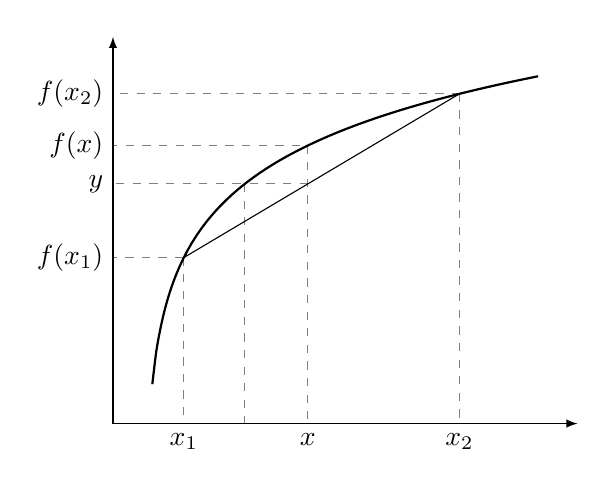
\begin{tikzpicture}[my plot/.style={
                        thick,
                        smooth,
                        samples=100,
                        domain=0.1:5},
                    my grid/.style={dashed,opacity=0.5, every node/.style={black,opacity=1}},
                    my axis/.style={latex-latex}]
\draw[my plot] (0,0) plot (\x,{ln(\x)});
\coordinate (start plot) at (0.1,{ln(0.1)}); % domain start
\coordinate (end plot) at (5,{ln(5)}); % domain end
\draw[my axis] ([shift={(-0.5cm,0.5cm)}]start plot |- end plot) node[left] {} |- node[coordinate](origin){} ([shift={(0.5cm,-0.5cm)}]start plot -| end plot) node[below] {}; %creates the axis a little bigger than the plot and also sepatared
\def\x{0.5}\def\y{4}\def\p{0.55} % define the x, y and p values
\coordinate (Ux) at (\x,{ln(\x)}); % set the u(x) coordinate
\coordinate (Uy) at (\y,{ln(\y)}); % set the u(y) coordinate
\coordinate (Up) at ({\p*\x+(1-\p)*\y},{ln(\p*\x+(1-\p)*\y)}); % set the u(p*x+(1-p)*y) coordinate
\draw (Ux) -- coordinate[pos=1-\p] (Up-mid) (Uy); % set the coordinate on the linear curve
\path let \p1=(Up-mid), \n1={pow(e,\y1*0.03514)} in (28.4576*\n1,\y1) coordinate (Up-mid2); %this is the most tricky part explained in the answer
% with everything set, just draw the lines:
\draw[my grid] (Ux) |- node[below]{$x_1$} (origin) |- node[left]{$f(x_1)$} cycle;
\draw[my grid] (Uy) |- node[below]{$x_2$} (origin) |- node[left]{$f(x_2)$} cycle;
\draw[my grid] (Up) |- node[below]{$x$} (origin) |- node[left]{$f(x)$} cycle;
\draw[my grid] (Up-mid2) |- node[below]{} (origin) |- node[left]{$y$} cycle;
\draw[my grid] (Up-mid) -- (Up-mid2);
\end{tikzpicture}
\end{center}
\end{annotation}


\begin{annotation}
\rm 我们这里使用的凹凸性都是描述函数性质的,并不是用来描述函数图像的,{\color{red}高数书使用的是对图像的凹凸性描述的},这里有几种记忆函数凹凸性质的方法.
\begin{enumerate}
	\item 从几何性质上,凹函数的曲线在两点确定的弦之上,凸函数的曲线在两点确定的弦之下.
\end{enumerate}	
\end{annotation}

\begin{theorem}
\rm {\color{red} (凹凸性判定1)} 给定在区间$\mathcal{X}$上定义着的连续可导函数$f(x)$,它是凸函数(凹函数)当且仅当它导数$f'(x)$是单调增的(单调减的). 
\end{theorem}

\begin{proof}
前面我们知道凸函数的性质可以用
$$
f(x) \leq \frac{x_2 - x}{x_2-x_1}f(x_1) + \frac{x-x_1}{x_2-x_1}f(x_2),\; x \in [x_1,x_2]
$$
来描述,来略微整理一下
$$
\begin{array}{ll}
&(x_2-x)f(x_1) + (x_1-x_2)f(x) + (x-x_1)f(x_2) \geq 0 \\ \\
\Rightarrow & (x_2 - x)(f(x_1)-f(x)) + (x_1 -x)(f(x)-f(x_2)) \leq  0 \\ \\
\Rightarrow & \frac{f(x) - f(x_1)}{x -x_1} \leq \frac{f(x_2) - f(x)}{x_2 - x} \\
\end{array}
$$
不等式两边在必要性证明中可以让$x$分别趋向$x_1$或者$x_2$求得
$$
f'(x_1) \leq \frac{f(x_2) - f(x_1)}{x_2 - x_1}
$$
和 
$$
f'(x_2) \geq \frac{f(x_2) - f(x_1)}{x_2 - x_1} 
$$
即有$f'(x_2) \geq f(x_1)$.

在充分证明中可以使用拉格朗日中值定理让等式两边分别等于$f(\xi_1)$和$f(\xi_2)$,其中$x_1 < \xi_1 < x < \xi_2 < x_2$.
\end{proof}


\begin{theorem}
\rm {\color{red} (凹凸性判定2)} 给定在区间$\mathcal{X}$上定义着的连续且二阶可导函数$f(x)$,它是凸函数(凹函数)当且仅当$f^{''}(x) \geq 0(\leq 0)$.
\end{theorem}

\begin{proof}
由单调性判定定理,回到前一个定理中的$f'(x)$的性质即可.
\end{proof}

\begin{theorem}
\rm {\color{red} (凹凸性判定3)} 给定在区间$\mathcal{X}$上定义着的连续可导函数$f(x)$,它是凸函数(凹函数)当且仅当它的曲线在它任意切线上面(切线下面).
\end{theorem}

\begin{proof}
{\color{blue}充分性} 任意点$x_0 \in \mathcal{X}$处切线方程$y = f(x_0) + f'(x)(x-x_0)$,那么只需要证明
$$
f(x) \leq f(x_0) + f'(x)(x-x_0) 
$$
当$x > x_0$时有
$$
f'(x_0) \geq \frac{f(x)-f(x_0)}{x-x_0}.
$$
当$x < x_0$时有
$$
f'(x_0) \leq \frac{f(x)-f(x_0)}{x-x_0}.
$$
那么根据拉格朗日中值定理可以找到$\xi_1 <x_0 < \xi_2$,使得
$$
f'(x_0) \leq f'(\xi_2),\; f'(x_0) \leq f'(\xi_1).
$$
即$f'(\xi_1) \leq f'(\xi_2)$,回到第一个判别定理.
\end{proof}

\begin{proposition}
\rm {\color{red} (琴生不等式)} 凸函数满足 
$$
f(q_1x_1 + q_2x_2 + \cdots + q_nx_n) \leq q_1f(x_1) +q_2f(x_2) + \cdots + q_nf(x_n),
$$
其中$q_1 + q_2 + \cdots + q_n = 1,\; q_1,q_2,\cdots,q_n > 0$.
\end{proposition}

\begin{definition}
\rm 若曲线$f(x)$在经过$(x_0,f(x_0))$时,曲线的凹凸性改变了,则这一点称为{\color{red}拐点}.
\end{definition}

\begin{proposition}
\rm {\color{red}判别拐点的存在方法}
\begin{enumerate}
	\item 若$f(x)$的二阶导存在,且$f(x)$在$x_0$处$f^{''}(x)=0$变号,则在$x_0$处有拐点.
	\item 若$f(x)$的$n$阶导数存在,如果点$x_0$处第一个不为零的导数(大于二阶导)是奇数阶导数,那么在$x_0$处有拐点,如果是偶数阶导数,则没有拐点.
\end{enumerate}
\end{proposition}

\newpage
\section{不定积分}

\subsection{不定积分定义}
\begin{definition}
\rm 若在给定的整个区间上,$f(x)$是函数$F(x)$的导数,或$f(x)dx$是$F(x)$的微分,即
$$
F'(x) = f(x)~\text{或}~dF(x) = f(x)dx,
$$
那么,在所给定的区间上,函数$F(x)$叫做$f(x)$的{\color{red}原函数}或者$f(x)$的{\color{red}积分}.
\end{definition}

\begin{theorem}
\rm {\color{red} (不定积分表达式) }若在某一个区间$\mathcal{X}$上,函数$F(x)$是$f(x)$的一个原函数,那么$F(x)+C$也是$f(x)$的原函数,其中$C$是任意常数. 反过来说,在区间$\mathcal{X}$上$f(x)$的每一个原函数都可表示这种形式.
\end{theorem}

\begin{proof}
记$\Phi(x)$是$f(x)$另一个原函数,则考虑辅助函数$\varphi(x) = \Phi(x) - F(x)$的导数
$$
(\Phi(x)-F(x))' = f(x)-f(x) = 0.
$$
由常函数判定定理,可以知道$\varphi(x) = C$,所以$\Phi(x) = F(x) + C$.
\end{proof}

\begin{definition}
\rm 在区间$\mathcal{X}$,函数$f(x)$的带任意常数项的原函数称为$f(x)$在$\mathcal{X}$上的{\color{red}不定积分},记做
$$
\int f(x)dx
$$
来表示,其中$f(x)$表示{\color{red}被积函数},乘积$f(x)dx$被称为{\color{red}被积表达式}.
\end{definition}

\begin{proposition}
\rm 从不定积分的定义可以很容易直接推导下面一些性质
\begin{enumerate}
	\item $d\int f(x)dx = f(x)dx,$
	\item $\int F'(x)dx = F(x)+C~\text{或}~\int dF(x) = F(x)+C.$
\end{enumerate}
\end{proposition}


\subsection{基本积分表}

\subsection{简单积分法则}

\begin{proposition}
\rm 简单法则
\begin{enumerate}
	\item 若$a$是常数且不等于0,则
	$$
	\int a\cdot f(x)dx = a \int f(x)dx,
	$$
	\item 
	$$
	\int \left[ f(x) \pm  g(x) \right]dx = \int f(x)dx + \int g(x)dx,
	$$
	\item 若$\int f(t)dt = F(t)+C$,则
	$$
	\int f(ax+b)dx = \frac{1}{a}\cdot F(ax+b)+C'
	$$
	{\color{red} 换元法则中极为特别的情形}
\end{enumerate}
\end{proposition}

\begin{proof}
{\color{blue}证明手法通常对右边取微分}.
\end{proof}


\subsection{换元积分法}
\begin{proposition}
\rm 如果已知
$$
\int g(t)dx = G(t)+C,
$$
即有
$$
\int g(\omega(x))\omega'(x)dx = G(\omega(x)) + C'.
$$
\end{proposition}

\begin{proof}
$$
\frac{d}{dx}G(\omega(x)) = G'(\omega(x))w'(x) = g(\omega(x))\omega'(x).
$$
\end{proof}

\begin{annotation}
\rm {\color{red} (换元积分法使用的直觉)} 要理解上述方法的先决条件,只需要关系式$dG(t)=g(t)dt$成立,就有上述换元之后的关系式存在. 现在换个思路,若先要计算积分
$$
\int f(x)dx,
$$
但是这个$f(x)$并不好直接利用现有的一些手法求出其原函数,若被积部分可以表示成前面第二个关系式的左边
$$
f(x)dx = g(\omega(x))\omega'(x)dx,
$$
那么说明其原函数可以表示$G(\omega(x))$,这样我们尝试先求出$G(t)$,现在我们让$t=\omega(x)$,上式就变成了$\int g(t)dt$,{\color{blue}最重要是需要它是可以稍微容易求解的形式,不然换元就没什么意义}. 那么把它积出来之后等于$G(t)+C$,之后我们只需要把$t$用$\omega(x)$替换即可,因此可以简单的写成
$$
\int f(x)dx = \int g(x)dx.
$$
\end{annotation}

\begin{example}
\rm 求积分
$$
\int \sin^3\cos xdx.
$$
设$t=\sin x$,那么原式为
$$
\int \sin^3x\cos xdx = \int \sin^3xd\sin x = \int t^3 dt = \frac{t^4}{t}+C.
$$
最后$t$替换为$\sin x$即可.
\end{example}

\subsection{分部积分法}

\begin{proposition}
\rm 设$u=f(x)$和$v=g(x)$都是两个关于$x$的连续可导的函数,则
$$
\int udv  = uv - \int vdu.
$$
\end{proposition}

\begin{proof}
根据微分乘法法则
$$
d(uv) = udv + udv,
$$
两边取积分得到原式.
\end{proof}

\begin{annotation}
\rm {\color{red} (分部积分使用注意)} 它进行如下转换
$$
f(x)dx = uv'dx = udv = uv-vdu = vu'dx.
$$
在应用分部积分的时候,需要注意以下几点
\begin{enumerate}
	\item 被积表达式$f(x)$要被分成两个因式$u$和$dv=v'dx$.
	\item 微分$vu'dx$要比原式更容易积分.
\end{enumerate}
\end{annotation}


\begin{example}
\rm 求积分
$$
\int x\cos xdx.
$$
设$u=x,\; v= \sin x$,那么原式变为
$$
\int xd\sin x = x\sin x - \int \sin x dx = x\sin x +\cos x + C.
$$
\end{example}


\begin{proposition}
\rm {\color{red} (分部积分的推广公式)} 若$u$和$v$在所考虑的区间上有直到$(n+1)$阶的各阶连续导数,那么可以用$v^{(n)}$替换前式中的$v$,则
$$
\int uv^{(n+1)}dx = \int udv^{(n)} = uv^{(n)} - \int v^{(n)}du = uv^{(n)} - \int u'v^{(n)}dx.
$$
类似的
$$
\begin{array}{ll}
\int u'v^{(n)}dx &= u'v^{(n-1)} - \int u^{''}v^{(n-1)}dx, \\
\int u^{''}v^{(n-1)}dx &= u^{''}v^{(n-2)} - \int u^{'''}v^{(n-2)}dx, \\
&\vdots \\
\int u^{(n)}v'dx &= u^{(n)}v - \int u^{(n+1)}vdx, \\
\end{array}
$$
因此最终可以得到
$$
\int uv^{(n+1)}dx = uv^{(n)} - u'v^{(n-1)} + u^{''}v^{(n-2)} -\cdots + (-1)^{n} u^{(n)}v +  (-1)^{n+1} \int u^{(n+1)}vdx.
$$
\end{proposition}

\begin{annotation}
\rm {\color{red} (推广式中的特殊情况) }特别地,如果$u$是$n$元多项式,那么在$n+1$次求导之后就变成零了,上式子的尾巴就消失了.
\end{annotation}

\begin{example}
\rm 求积分
$$
J_n = \int \frac{1}{(x^2+a^2)^n}dx,\; n =1,2,3,\cdots.
$$
令$u=\frac{1}{(x^2+a^2)^n},\; v = x$,即
$$
J_n = \int \frac{1}{(x^2+a^2)^n}dx = \frac{x}{(x^2+a^2)^n} + 2n \int \frac{x^2}{(x^2+a^2)^{n+1}}dx. 
$$
考虑右式最后一项
$$
\int \frac{x^2}{(x^2+a^2)^{n+1}}dx =\int \frac{(x^2+a^2) - a^2}{(x^2+a^2)^{n+1}}dx = J_n - a^2 J_{n+1}.
$$
带入原式
$$
J_n = \frac{x}{(x^2+a^2)^n}+2nJ_n - 2a^2nJ_{n+1},
$$
整理得到{\color{red}递归式}
$$
J_{n+1} = \frac{1}{a^2}\frac{2n-1}{2n}J_n + \frac{1}{2a^2}\frac{1}{n}\frac{x}{(x^2+a^2)^n}.
$$
易得$J_1 = \frac{1}{a} \arctan \frac{x}{a}.$ 
\end{example}

\subsection{有理式积分}

\begin{annotation}
\rm 在各类函数的积分中使我们{\color{red}最感兴趣的是什么},要根据什么样的{\color{red}法则},才能得到它们的积分,是这一节我们主要关注的问题. 积佬养成)
\end{annotation}

\begin{definition}
\rm 形如
$$
f(x)=\frac{P(x)}{Q(x)}
$$
的函数,其中$P(x),Q(x)$均为多项式. 这样的函数被称为{\color{red}有理函数}.
\end{definition}

\begin{proposition}
\rm 两种{\color{red}简单真分式}积分方法
\begin{enumerate}
	\item $\frac{A}{x-a}$
	$$
	A\int \frac{1}{x-a}dx = A \ln(x-a) + C.
	$$
	\item $\frac{A}{(x-a)^k},\; k = 2,3,\cdots$
	$$
	A\int \frac{1}{(x-a)^k}dx = -\frac{A}{k-1}\frac{1}{(x-a)^{k-1}} + C
	$$
\end{enumerate}
\end{proposition}

\begin{annotation}
\rm {\color{red}(部分分式)}求积分
$$
\int \frac{Mx+N}{(x^2+px+q)^m}dx,\; m = 2,3,4,\cdots.
$$
同时假定$x^2+px+q$没有实根,即$p^2 - 4q < 0$.

先对分母括号中的二次多项式进行配方
$$
\begin{array}{ll}
\int \frac{Mx+N}{(x^2+px+q)^m}dx &= \int \frac{Mx+N}{(x^2+2\frac{p}{2}x+\frac{p^2}{4}-\frac{p^2}{4}+q)^m}dx\\
&= \int \frac{Mx+N}{\left[(x+\frac{p}{2})^2+(q-\frac{p^2}{4})\right]^m}dx
\end{array}
$$
设$x+\frac{p}{2} = t, a = + \sqrt{q-\frac{p^2}{4}}$,现在$dt=dx$,那么原式变为
$$
\int \frac{M(t-\frac{p}{2})+N}{\left(t^2+a^2\right)^m}dt = M\int \frac{t}{\left(t^2+a^2\right)^m}dt + (N-\frac{Mp}{2})\int \frac{1}{\left(t^2+a^2\right)^m}dt,
$$
等式右边第一个积分,设$t^2+a^2 = u$,那么其积分变为
$$
M\int \frac{t}{\left(t^2+a^2\right)^m}dt = \frac{M}{2} \int  \frac{du}{u^m} = \frac{M}{2} \frac{-1}{m-1}\frac{1}{u^{m-1}} + C = \frac{-M}{2(m-1)}\frac{1}{(t^2+a)^{m-1}}+C.
$$
右边第二个积分使用我们在分部积分里面提到的{\color{blue}递归式求解}即可. 
\end{annotation}

\begin{theorem}
\rm 每个真分式
$$
\frac{P(x)}{Q(x)}
$$
可被表示成{\color{red}有限个部分分式的代数和}的形状. {\color{blue}总感觉有点环上PID性质在里面??????}
\end{theorem}

\begin{proof}
首先我们需要知道任意一个多项式的分解可以写成下述形式
$$
Q(x) = (x-a)^k \cdots (x^2+px+q)^m \cdots,\; k,m \in \mathbb{N},\; a,p,q \in \mathbb{R},
$$
其中$x^2+px+q$没有实根,相当于在实数环上做因式分解. 下面分两种情况来讨论$\frac{P(x)}{Q(x)}$的部分分式. 

{\color{blue}(1)} 若所给真分式为
$$
\frac{P(x)}{Q(x)} = \frac{P(x)}{(x-a)^kQ_1(x)}.
$$
则可以表示成下述两个真分式的和
$$
\frac{P(x)}{(x-a)^kQ_1(x)} = \frac{A}{(x-a)^k} + \frac{P_1(x)}{(x-a)^{k-1}Q_1(x)},
$$
其中$A$是一个常量,接下来就是确定$A$和$P_1(x)$,即这里有一个恒等式
$$
P(x) = AQ_1(x) + P_1(x)(x-a).
$$
首先我们得确定这里有解才行,{\color{blue}注意这里$(x-a)$和$Q_1(x)$是互素的,但是不能直接用Bezout定理说明这里有解,因为这里限定$A$是一个常量而不是一个关于$x$的多项式}. 那么现在问题变成了要说明其中一个解是常量,是这样的因为Bezont定理,我们得到这样一个等式
$$
u(x)Q_1(x) + v(x)(x-a) = 1.
$$
可以来尝试把所有$Q_1(x)$和$(x-a)$线性组合为$1$的系数用$u(x)$和$v(x)$表示出来,即
$$
U(x) = u(x) - (x-a)t(x),\; V(x) = v(x) - Q_1(x)t(x). 
$$
我们主要关注$U(x)$来说明一定可以取到常数$A$,相当于$U(x)$可以是$u(x)$除$(x-a)$的余数,所以$U(x)$是一定可以取到某个常数$A$.自然地,这里考虑可以取$x = a$消去含$P_1(x)$的项,于是得到$A=\frac{P(a)}{Q_1(a)}$,随之再确定$Q_1(a)$. 记录一个我自己的疑问{\color{red}为什么给定真分式不能分解为}
$$
\frac{A}{(x-a)^k} + \frac{B}{Q_1(x)},\; k=2,3,\cdots,
$$
那么确定的恒等式就变成了
$$
P(x) = AQ_1(x) + B(x-a)^k, 
$$
按照前面的思路这里$U(x) = u(x) - (x-a)^kt(x)$,所以只能保证$U(x)$取到某个$a_{k-1}x^{k-1}+a_{k-2}x^{k-2}+\cdots+a_0$,那么这里$A$可能就不一定是一个常数.

{\color{blue}(2)} 若所给真分式为
$$
\frac{P(x)}{Q(x)} = \frac{P(x)}{(x^2+px+q)^mQ_1(x)}.
$$
则可以表示成下述两个真分式的和
$$
\frac{P(x)}{(x+px+q)^mQ_1(x)} = \frac{Mx+N}{(x^2+px+q)^m} + \frac{P_1(x)}{(x^2+px+q)^{m-1}Q_1(x)}.
$$
其中$M,N,P_1(x)$确定要稍微复杂一点,但是整体思路是明确的,详细参考菲砖对应有理分式积分章节.

上面两种情况的尾巴均可以再依次取类似的部分分式,即
$$
\frac{A_1}{x-a} + \frac{A_2}{(x-a)^2} + \cdots + \frac{A_k}{(x-a)^k}.
$$
和
$$
\frac{M_1x+N_1}{x^2+px+q} + \frac{M_2x+N_1}{(x^2+px+q)^2} + \cdots + \frac{M_{m}x+N_{m}}{(x^2+px+q)^m}.
$$
对其部分分式代数和进行积分将比原始要简单的多! 但是这里只是证明某个真分式可以被表示成有限个部分分式,但是具体相关的系数其实都只是指称,若展开成代数和形式之后,求相关的系数方法,我们称其为{\color{red}待定系数法}.
\end{proof}


\begin{example}
\rm 求下列给定分式的分解式
$$
\frac{2x^2+2x+13}{(x-2)(x^2+1)^2}
$$
原式的分解形式可以先写成如下形式
$$
\frac{A}{x-2} + \frac{Bx+C}{x^2+1} + \frac{Dx+E}{(x^2+1)^2}.
$$
其中$A,B,C$就是待定系数,它和原式关系等式为
$$
\begin{array}{ll}
2x^2 + 2x+ 13 &= A(x^2+1)^2 + (Bx+C)(x-2)(x^2+1) + (Dx+E)(x-2) \\
			  &= (A+B)x^4 + (C-2B)x^3 + (2A+B-2C+D)x^2 + (C-2B-2D+E)x + (A-2C-2E).
\end{array}
$$
这里对应一个含5个方程的方程组
$$
\left\{ 
\begin{array}{ll}
A+B &= 0 \\
C-2B &= 0 \\
2A+B-2C+D &= 2 \\
C-2B-2D+E &= 2 \\
A-2C-2E &= 13  
\end{array}
\right.
$$
解这个方程组可以先利用后三项消去$D,F$得到一个只含$A,B,C$的等式,再配合前两项,先解出$A,B,C$. 由此
$$
A = 1,\;B = -1,\;C = -2,\;D = -3 ,\;E=-4.
$$
最后
$$
\frac{2x^2+2x+13}{(x-2)(x^2+1)^2} = \frac{1}{x-2} + \frac{-x-2}{x^2+1} + \frac{-3x-4}{(x^2+1)^2}.
$$
\end{example}

\newpage
\section{定积分}

\subsection{定积分定义}

\begin{definition}
\rm 给定定义在区间$[a,b]$上的函数$f(x)$. 在$a$和$b$之间插入若干分点
$$
a = x_0 < x_1 <x_2 < \cdots < x_{n-1} < x_n = b
$$
把$[a,b]$分成$n$个小区间
$$
[x_0,x_1],[x_1,x_2],\cdots,[x_{n-1},x_n].
$$
用$\Delta x_i = x_{i+1}-x_i$第$i$小区间的长度,记$\lambda = \max{\{\Delta x_i\}}$. 从每个小区间$[x_i,x_{i+1}]$上任取一点$x=\xi_i$并做出和
$$
\sigma = \sum\limits_{i=0}^{n-1}f(\xi_i)\Delta x_i.
$$
若$\lambda \rightarrow 0$时$\sigma$有有限极限$I$,用极限的语言描述即对任意的$\varepsilon > 0$,都可以找到数$\delta$,只要$\lambda < delta$,不等式
$$
|\sigma - I| < \varepsilon
$$
在任意的$\xi_i$选择之下皆成立,把其记做
$$
I = \lim\limits_{\lambda \rightarrow 0} \sigma.
$$
则这极限$I$叫做函数$f(x)$在从$[a,b]$上的{\color{red}定积分},记为
$$
I = \int_a^b f(x)dx.
$$
在这情形下$f(x)$叫做$[a,b]$上的{\color{red}可积函数},数$a$与$b$分别叫做积分的{\color{red}上限}和{\color{red}下限},区间$[a,b]$,叫做{\color{red}积分区间},变量$x$叫做{\color{red}积分变量}. $\sigma$也被称为{\color{red}黎曼和},上述定义本身就是{\color{red}黎曼定义}.
\end{definition}

\subsection{定积分基本性质}

\begin{proposition}
\rm {\color{red} (可积的必要条件)} 可积函数一定是有界的.
\end{proposition}

\begin{definition}
\rm 用$m_i$与$M_i$分别表示函数$f(x)$在第$i$个部分区间$[x_i,x_{i+1}]$上的下确界和上确界,并作和
$$
s = \sum\limits_{i=0}^{n-1}m_i\Delta x_i,\; S = s = \sum\limits_{i=0}^{n-1}M_i\Delta x_i
$$
这两个和分别叫做{\color{red}下积分}和与{\color{red}上积分和},或者{\color{red}达布和}. 当$f(x)$连续时,$f(x)$在每个区间上都能去掉确界,于是
$$
m_i \leq f(\xi_i) \leq M_i,
$$ 
自然地也有
$$
s \leq \sigma \leq S.
$$
这意味着$s$与$S$分别是积分和的下确界与上确界.
\end{definition}


\begin{lemma}
\rm 如果把一些新的点加入到已有的分点中,即插入$x'$位于任意的部分区间$[x_k,x_{k+1}]$有$x_k < x' < x_{k+1}$. 则达布下和只有可能因此增加,而上和只可能减少.
\end{lemma}

\begin{proof}
一个小区间被分成了两个更小的区间,这两个更小区间的积分和加起来是小于原先区间的积分和.
\end{proof}

\begin{lemma}
\rm 任何一个达布下和都不超过任何一个上和,即使是对应于区间的另一个划分的上和,即两个不同的区间划分构造$s_1,S_2$和$s_2,S_2$,也有$s_1 < S_2$.
\end{lemma}

\begin{proof}
通过第一个lemma,通过加点的方式,联合两个构造组成一个新的构造$s_3,S_3$,因此有$s_1 \leq s_3$和$S_2 \geq S_3$,且有$s_3 \leq S_3$,所以$s_1 \leq S_2$.
\end{proof}

\begin{theorem}
\rm {\color{red}定积分存在的充要条件}是
$$
\lim\limits_{\lambda \rightarrow 0} (S-s) = 0.
$$
设$\omega_i$为第$i$区间上的{\color{red}振幅}$M_i - m_i$,那么上述式子也可以表示成
$$
\lim\limits_{\lambda \rightarrow 0} (S-s) = \sum\limits_{i=0}^{n-1} (M_i-m_i) \Delta x_i = \sum\limits_{i=0}^{n-1} \omega_i \Delta x_i = 0.
$$
\end{theorem}

\begin{proof}
{\color{blue} 必要性} 由极限定义
$$
I-\varepsilon \leq s \leq \sigma \leq S \leq I+\varepsilon.
$$
可以马上得到$|S-s| \leq \varepsilon$.

{\color{blue} 充分性} 由前一个lemma,可以知道所有的达布下积分都有上界,取对应的上确界为$I_*$; 下积分都有下界,取对应的下确界为$I^*$. 命题条件说明当$\lambda \rightarrow 0$时,有$I_* = I^*$,设其公共值为$I$,即有
$$
s \leq I \leq S,
$$
同时也有
$$
s \leq \sigma \leq S,
$$
自然地,在$\lim\limits_{\lambda \rightarrow 0} (S-s) = 0$极限意义下,有$|\sigma -I| < \varepsilon$.
\end{proof}


\begin{theorem}
\rm {\color{red} (可积的判别条件1) }如果函数$f(x)$在区间$[a,b]$上是连续的,则函数$f(x)$是可积的.
\end{theorem}

\begin{proof}
由函数在闭区间上连续,可知$f(x)$在$[a,b]$上一致连续,由其推论可知,给定任意$\varepsilon > 0$,能找到$\delta > 0$,使得把$[a,b]$分隔若干长度$\Delta x_i$小于$\delta$的小区间,则小区间上函数值的振幅小于$\varepsilon$,其用语言描述就是
$$
\sum\limits_{i=0}^{n-1} \omega_i \Delta x_i  \sum\limits_{i=0}^{n-1} \varepsilon \Delta x_i = \varepsilon(b-a).
$$
最后需要回顾极限的定义上,这里只有$\lambda < \delta$,我们再需要说明一下当满足前面条件的同时$\lambda \rightarrow 0$,积分和保持是小于$\sum\limits_{i=0}^{n-1} \varepsilon \Delta x_i$,这是显然的,使用在证明lemma 10.4中的手法说明即可.
\end{proof}

\begin{theorem}
\rm {\color{red} (可积的判别条件2) } 若在区间$[a,b]$上的有界函数$f(x)$只有有限多个间断点,则它是可积的.
\end{theorem}

\begin{proof}
在间断点处划分区间,详细证明见菲砖.
\end{proof}

\begin{theorem}
\rm {\color{red} (可积的判别条件3) } 在$[a,b]$单调有界函数$f(x)$永远可积.
\end{theorem}

\begin{proof}
方便证明设$f(x)$是单调增函数,那么在部分区间$[x_i,x_{i+1}]$上,其振幅为
$$
\omega_i = f(x_{i+1})-f(x_{i}).
$$
对于任意的$\varepsilon > 0$,我们让
$$
\delta = \frac{\varepsilon}{f(b)-f(a)}.
$$
使得$f(b)\neq f(a)$,不然常函数肯定可积. 再让$\lambda < \delta$那么
$$
\sum\limits_{i=0}^{n-1}\omega_i\Delta x_i < \sum\limits_{i=0}^{n-1}\left[f(x_{i+1})-f(x_{i})\right] \delta = \delta\left[ f(b)-f(a) \right] 
$$
由此可推导$f(x)$可积.
\end{proof}

\begin{proposition}
\rm {\color{red}可积函数的一些性质}
\begin{enumerate}
	\item 若$f(x)$在区间$[a,b]$上可积,则函数$|f(x)|$和$kf(x)$($k$是任意常数)在这区间上也是可积的.
	\item 若$f(x)$和$g(x)$在区间$[a,b]$上是可积的,则它们的和,差与乘积也是可积的.
	\item 若$f(x)$在区间$[a,b]$上可积,则它在这区间上的任意一个部分区间$[\alpha,\beta]$都是可积的. 反之如果区间$[a,b]$被分割成了若干部分区间,并且分别在每个部分区间上$f(x)$是可积,则它在整个区间$[a,b]$也是可积的.
	\item 如果改变可积函数在有限个点上的值,则它的可积性并不会被破坏. {\color{blue} 即使$f(x)$在区间$[a,b]$的有限个点上不确定时,我们也可以谈论积分$\int_a^b f(x)dx$. 同时可以在这些点处给定它们任意的函数值而考虑整个区间上的积分. 如我们已经见到的,无论积分是否存在,或是它的值都不依赖在那些不存在函数的点处我们加上的函数值}.
\end{enumerate}
\end{proposition}

\begin{proof}
特别地说明一下(4), 为什么在{\color{red}改变有限个函数值之后积分结果不变}? 考虑积分定义
$$
\int_a^b f(\xi_i)\Delta x_idx,
$$ 
由于$f(x)$本身的可积性,保证了我们任取$\xi_i$最后极限都是一样的,那么当我们改变了有限个函数值之后,上面和式中的只有有限项会被影响,针对这有限项我们只需要在选择$\xi_i$的时候避开其改变了函数值的那些点,最后还是可以保证极限.
\end{proof}

\begin{proposition}
\rm {\color{red}定积分的一些性质} 若$f(x)$在$[a,b]$上可积
\begin{enumerate}
	\item 
	$$
	\int_a^b f(x)dx = - \int_b^a f(x)dx.
	$$
	\item 若$a<c<b$,则
	$$
	\int_a^b f(x)dx  = \int_a^c f(x)dx + \int_c^b f(x)dx.
	$$
	\item 给定常数$k$,则
	$$
	\int_a^b kf(x)dx = k \int_a^b f(x)dx.
	$$
	\item 若$g(x)$也在$[a,b]$上可积,则
	$$
	\int_a^b f(x)\pm g(x)dx = \int_a^b f(x)dx \pm \int_a^b g(x)dx.
	$$
	\item 若$f(x)$在$[a,b]$非负,则
	$$
	\int_a^b f(x)dx \geq 0.
	$$
	\item 若$g(x)$也在$[a,b]$上可积,且恒有$g(x) \geq f(x)$,则
	$$
	\int_a^b f(x)dx \leq \int_a^b g(x)dx.
	$$
	\item 
	$$
	\left|\int_a^b f(x)dx\right| \leq \int_a^b |f(x)|dx.
	$$
	\item 若在$[a,b]$上有$m \leq f(x) \leq M$,则
	$$
	m(b-a) \leq \int_a^b f(x)dx \leq M(b-a).
	$$
\end{enumerate}
\end{proposition}


\begin{theorem}
\rm {\color{red} (积分中值定理) } 若$f(x)$在$[a,b]$上可积,在整个区间上都有$m \leq f(x) \leq M$,则
$$
\int_a^b f(x)dx = \mu(b-a),
$$
其中$m\leq \mu \leq M$. 特别地当$f(x)$连续时,存在一点$c\in [a,b]$使得$u=f(c)$.  
\end{theorem}

\begin{proof}
根据前面性质(8),有
$$
m \leq \frac{1}{b-a}\int_a^b f(x)dx \leq M \\
$$
令
$$
\frac{1}{b-a}\int_a^b f(x)dx = u,
$$
即马上可以得到命题中的结论.
\end{proof}

\begin{theorem}
\rm {\color{red} 推广中值定理} (1)$f(x)$和$g(x)$在区间$[a,b]$上可积;(2)$m\leq f(x) \leq M$;(3) $g(x)$在整个区间上不变号,即$g(x) \leq 0$或者$g(x) \geq 0$. 则
$$
\int_a^b f(x)g(x)dx = u\int_a^b g(x)dx.
$$
特别地当$f(x)$连续时,存在一点$c\in [a,b]$使得$u=f(c)$.  
\end{theorem}
\end{document}

